%%%%%%%%%%%%%%%%%%%%%%%%%%%%%%%%%%%%%%%%%%%%%%%%%%%%%%%%%%%
%
%    Basierend auf der Vorlage von Prof. Braun, FHWS
%
%%%%%%%%%%%%%%%%%%%%%%%%%%%%%%%%%%%%%%%%%%%%%%%%%%%%%%%%%%%
\documentclass[12pt,oneside,numbers=noenddot,a4paper,parskip]{scrbook}
\usepackage[utf8]{inputenc}
\usepackage{xargs}
\usepackage{wrapfig}
\usepackage{csquotes}
\usepackage[ngerman]{babel}
\usepackage{subfigure}
\usepackage[pdftex]{graphicx}
\usepackage{pgfgantt}
\usepackage[hidelinks]{hyperref}
\usepackage{color}
\usepackage{amssymb}
\usepackage{textcomp}
\usepackage{pdfpages}
\usepackage{array}
\usepackage{multirow}
\usepackage{float}
\usepackage{pdflscape}
\usepackage{everypage}
\usepackage{lipsum}
\usepackage{lscape}
\usepackage{subfigure}
\usepackage{pdfpages}  
\usepackage[verbose]{placeins} 
\usepackage[nouppercase,headsepline,plainfootsepline]{scrpage2}
\usepackage{listings}		
\usepackage{xcolor}
\usepackage{geometry}
\usepackage{color}			
\usepackage[hypcap]{caption}
\usepackage{subfigure}			
\usepackage{epstopdf}		
\usepackage{tabularx}  
\usepackage{setspace}
\usepackage{booktabs}
\setcounter{secnumdepth}{2}
\usepackage[style=numeric,backend=bibtex,sorting=none]{biblatex}
\setcounter{tocdepth}{2}
%%%%%%%%%%%%%%%%%%%%%%%%%%%%%%%
%    Literatur File           %
%%%%%%%%%%%%%%%%%%%%%%%%%%%%%%%
\bibliography{literatur}            

%%%%%%%%%%%%%%%%%%%
%% definitions
%%%%%%%%%%%%%%%%%%%
\def\BaAuthor{Frank Rügamer \& Co.}
\def\BaTitle{
\includegraphics[width= 0.6\textwidth]{resources/SM_logo_start}}
\def\BaSupervisorTwo{Prof.\ Dr.\ Steffen Heinzl}
\def\BaSupervisorOne{Vitaliy Schreibmann}
\def\BaDeadline{\today}

\hypersetup{
pdfauthor={\BaAuthor},
pdftitle={\BaTitle},
pdfsubject={Subject},
pdfkeywords={Keywords}
}

%%%%%%%%%%%%%%%%%%%
%% macros to include
%%%%%%%%%%%%%%%%%%%
\newcommand{\frank}{Frank Rügamer}
\newcommand{\leonard}{Leonard Nickels}
\newcommand{\oliver}{Oliver Gawron}
\newcommand{\philipp}{Philipp Jung}

% Author hint for chapters
\makeatletter
\newcommand{\chapterauthor}[1]{%
	{\parindent0pt\vspace*{-40pt}%
		\linespread{1.1}\hspace*{29pt}\large\scshape#1%
		\par\nobreak\vspace*{5pt}}
	\@afterheading%
}
\makeatother


% Author hint for sections
\makeatletter
\newcommand{\sectionauthor}[1]{%
	{\parindent0pt\vspace*{-30pt}%
		\linespread{1.1}\hspace*{33pt}\large\scshape#1%
		\par\nobreak}
	\@afterheading%
}
\makeatother


% Author hint for subsections
\makeatletter
\newcommand{\subsectionauthor}[1]{%
	{\parindent0pt\vspace*{-26pt}%
		\linespread{1.1}\hspace*{41pt}\large\scshape#1%
		\par\nobreak\vspace*{5pt}}
	\@afterheading%
}
\makeatother

% Author hint for subsections
\makeatletter
\newcommand{\subsubsectionauthor}[1]{%
	{\parindent0pt\vspace*{-26pt}%
		\linespread{1.1}\large\scshape#1%
		\par\nobreak\vspace*{5pt}}
	\@afterheading%
}
\makeatother

\usepackage[colorinlistoftodos,prependcaption,textsize=tiny]{todonotes}
\newcommandx{\unsure}[2][1=]{\todo[linecolor=red,backgroundcolor=red!25,bordercolor=red,#1]{#2}}
\newcommandx{\change}[2][1=]{\todo[linecolor=blue,backgroundcolor=blue!25,bordercolor=blue,#1]{#2}}
\newcommandx{\info}[2][1=]{\todo[linecolor=OliveGreen,backgroundcolor=OliveGreen!25,bordercolor=OliveGreen,#1]{#2}}
\newcommandx{\improvement}[2][1=]{\todo[linecolor=Plum,backgroundcolor=Plum!25,bordercolor=Plum,#1]{#2}}
\newcommandx{\thiswillnotshow}[2][1=]{\todo[disable,#1]{#2}}


\newcommand{\toremove}[1]{
	\textcolor{red}{#1}
}
\definecolor{InfBoxBorder}{rgb}{0.55,0.55,0.55}
\definecolor{InfBoxTop}{rgb}{0.75,0.75,0.75}
\definecolor{InfBoxBg}{rgb}{0.95,0.95,0.95}

% erstellt die box mit "ACHTUNG!" ueber dem eigentlichen text

% das "hint" environment fuer eine tolle box :)
\makeatletter\newenvironment{hintbox}%
{\fcolorbox{InfBoxBorder}{InfBoxTop}{\parbox{\textwidth}{\begin{minipage}{4.5mm}\vspace{-0.2mm}
\includegraphics[height=4.5mm]{macros/hint.pdf}\end{minipage}\textbf{Hinweis}}}\vspace{-1mm}\\\begin{lrbox}{\@tempboxa}\begin{minipage}{\textwidth}}
{\end{minipage}\end{lrbox}\fcolorbox{InfBoxBorder}{InfBoxBg}{\usebox{\@tempboxa}} }
\makeatother

%%%%%%%%%%%%%%%%%%%
%% configs to include
%%%%%%%%%%%%%%%%%%%
\colorlet{punct}{red!60!black}
\definecolor{background}{HTML}{EEEEEE}
\definecolor{delim}{RGB}{20,105,176}
\colorlet{numb}{magenta!60!black}

\definecolor{gray}{rgb}{0.4,0.4,0.4}
\definecolor{darkblue}{rgb}{0.0,0.0,0.6}
\definecolor{cyan}{rgb}{0.0,0.6,0.6}

\definecolor{pblue}{rgb}{0.13,0.13,1}
\definecolor{pgreen}{rgb}{0,0.5,0}
\definecolor{pred}{rgb}{0.9,0,0}
\definecolor{pgrey}{rgb}{0.46,0.45,0.48}

\usepackage{calc} 

\newlength\tdima 
\newlength\tdimb 
\newlength\offset
\setlength\offset{6pt}
\setlength\tdima{ \fboxsep+\fboxrule} 
\setlength\tdimb{-\fboxsep+\fboxrule+\offset} 


\definecolor{listinggray}{gray}{0.6}

\DeclareCaptionFont{white}{\color{white}}
\DeclareCaptionFormat{listing}{%
  \parbox{\textwidth}{\colorbox{listinggray}{\parbox{\textwidth-\offset}{#1#2#3}}\vskip+3pt}}
\captionsetup[lstlisting]{format=listing,labelfont=white,textfont=white}
\lstset{
frame = tlbr, %
columns=fullflexible, %
 basicstyle=\scriptsize\ttfamily,
 xleftmargin = \tdima, %
 xrightmargin = \tdimb, %
 tabsize=4, %
 language=Java, %
 upquote=false, %
 numberfirstline=true, %
 numberblanklines=false, %
 numbers=left,%
 numberstyle=\tiny, % 
 stepnumber=1, %
 numbersep = 10pt, %
 float=tp, %
 breakautoindent = true,%
 %This tells latex to keep more distance to the element above
 %aboveskip={1.5\baselineskip}, 
 showstringspaces=false, %
 extendedchars=true,%
 prebreak = \raisebox{0ex}[0ex][0ex]{\ensuremath{\hookleftarrow}}, %
 showtabs=false, %
 showspaces=false,%
 linewidth=\textwidth,%
 showstringspaces=false, %
 identifierstyle=\ttfamily, %
 keywordstyle=\color[rgb]{0,0,1}, %
 commentstyle=\color{gray}\upshape
 stringstyle=\color{black}, %
 breaklines=true, %
 breakatwhitespace=true, %
 columns=fullflexible, % 
 xleftmargin=8.9mm,%                 % code einrücken (rückt nummern mit ein!)
 framexleftmargin=22pt,%                % box so schieben, dass nummern mit drin sind
 framexrightmargin = 0pt, %
 escapechar=\&,						% char to escape out of listings and back to LaTeX
 literate={«}{{\flqq{}}}1 {»}{{\frqq{}}}1 %
} 
\lstdefinelanguage{JavaScript}{
	basicstyle=\scriptsize\ttfamily,
	keywords={typeof, new, true, false, catch, function, null, catch, switch, var, if, in, while, do, else, case, break, this},
	keywordstyle=\color{blue}\bfseries,
	ndkeywords={class, export, boolean, throw, implements, import, return},
	ndkeywordstyle=\color{red}\bfseries,
	identifierstyle=\color{black},
	sensitive=false,
	comment=[l]{//},
	morecomment=[s]{/*}{*/},
	commentstyle=\color{purple}\ttfamily,
	stringstyle=\color{red}\ttfamily,
	morestring=[b]',
	morestring=[b]"
}
\lstdefinelanguage{json}{
	basicstyle=\scriptsize\ttfamily,
    numbers=left,
    numberstyle=\scriptsize,
    stepnumber=1,
    numbersep=8pt,
    showstringspaces=false,
    breaklines=true,
    backgroundcolor=\color{background},
    literate=
     *{0}{{{\color{numb}0}}}{1}
      {1}{{{\color{numb}1}}}{1}
      {2}{{{\color{numb}2}}}{1}
      {3}{{{\color{numb}3}}}{1}
      {4}{{{\color{numb}4}}}{1}
      {5}{{{\color{numb}5}}}{1}
      {6}{{{\color{numb}6}}}{1}
      {7}{{{\color{numb}7}}}{1}
      {8}{{{\color{numb}8}}}{1}
      {9}{{{\color{numb}9}}}{1}
      {:}{{{\color{punct}{:}}}}{1}
      {,}{{{\color{punct}{,}}}}{1}
      {\{}{{{\color{delim}{\{}}}}{1}
      {\}}{{{\color{delim}{\}}}}}{1}
      {[}{{{\color{delim}{[}}}}{1}
      {]}{{{\color{delim}{]}}}}{1},
}


\lstdefinelanguage{CSharp}{
	basicstyle=\scriptsize\ttfamily,
    numbers=left,
    numberstyle=\scriptsize,
    stepnumber=1,
    numbersep=8pt,
    showstringspaces=false,
    breaklines=true,
    backgroundcolor=\color{background},
	morecomment = [l]{//}, 
	morecomment = [l]{///},
	morecomment = [s]{/*}{*/},
	morestring=[b]", 
	sensitive = true,
	morekeywords = {abstract,  event,  new,  struct,
		as,  explicit,  null,  switch,
		base,  extern,  object,  this,
		bool,  false,  operator,  throw,
		break,  finally,  out,  true,
		byte,  fixed,  override,  try,
		case,  float,  params,  typeof,
		catch,  for,  private,  uint,
		char,  foreach,  protected,  ulong,
		checked,  goto,  public,  unchecked,
		class,  if,  readonly,  unsafe,
		const,  implicit,  ref,  ushort,
		continue,  in,  return,  using,
		decimal,  int,  sbyte,  virtual,
		default,  interface,  sealed,  volatile,
		delegate,  internal,  short,  void,
		do,  is,  sizeof,  while,
		double,  lock,  stackalloc,   
		else,  long,  static,   
		enum,  namespace,  string, get, set}
}

\lstset{language=xml,
  morestring=[b]",
  morestring=[s]{>}{<},
  morecomment=[s]{<?}{?>},
  stringstyle=\color{black},
  numbers=left,
  numberstyle=\scriptsize,
  stepnumber=1,
  numbersep=8pt,
  identifierstyle=\color{darkblue},
  keywordstyle=\color{cyan},
  backgroundcolor=\color{background},
  morekeywords={xmlns,version,type}% list your attributes here
}

\lstset{language=Java,
  showspaces=false,
  showtabs=false,
  tabsize=4,
  breaklines=true,
  keepspaces=true,      
  numbers=left,
  numberstyle=\scriptsize,
  stepnumber=1,
  numbersep=8pt,
  showstringspaces=false,
  breakatwhitespace=true,
  commentstyle=\color{pgreen},
  keywordstyle=\color{pblue},
  stringstyle=\color{pred},
  basicstyle=\scriptsize\ttfamily,
  backgroundcolor=\color{background},
%  moredelim=[il][\textcolor{pgrey}]{$$},
%  moredelim=[is][\textcolor{pgrey}]{\%\%}{\%\%}
}
\newcolumntype{C}[1]{>{\centering\arraybackslash}m{#1}}
\geometry{a4paper, top=28mm, left=28mm, right=28mm, bottom=28mm, footskip=18mm}
\begin{document}

%%%%%%%%%%%%%%%%%%%
%% Titelseite
%%%%%%%%%%%%%%%%%%%


\frontmatter
\titlehead{%  {\centering Seitenkopf}
  {Hochschule für angewandte Wissenschaften Würzburg-Schweinfurt\\
   Fakultät Informatik und Wirtschaftsinformatik}}
\subject{Dokumentation Programmierprojekt}
\title{\BaTitle\\[15mm]}
\author{\BaAuthor}
\date{\normalsize{Eingereicht am: \today}}
\publishers{
  \normalsize{Betreuer: \BaSupervisorOne}\\
  \normalsize{Zweitpr\"{u}fer: \BaSupervisorTwo}\\
}

%\uppertitleback{ }
%\lowertitleback{ }

\maketitle


%%%%%%%%%%%%%%%%%%%
%% abstract
%%%%%%%%%%%%%%%%%%%

%%%%%%%%%%%%%%%%%%%
%% Inhaltsverzeichnis
%%%%%%%%%%%%%%%%%%%
\tableofcontents										



%%%%%%%%%%%%%%%%%%%
%% Main part of the thesis
%%%%%%%%%%%%%%%%%%%
\mainmatter

\section{Einleitung}

\subsection{Unterpunkt}
Mindestens 2 Unterpunkte oder keiner
\subsubsection{UnterUnterPunkt}

\paragraph{Sowas wie UnterUnterPunkt}
\chapter{Grundlagen}

\section{JDroid Library}
\sectionauthor{\philipp}

Die wichtigste Komponente der Kartenspiele ist die JDroid library. Die von
\href{http://www.aplu.ch/home/apluhomex.jsp?site=99}{Äegidius Plüss} entwickelte
Java Bibliothek implementiert ebenfalls die JCardGame Bibliothek für Android,
welche grundlegend für unsere Kartenspiele ist. Sie verfügt über eine
ausführliche
\href{http://www.java-online.ch/gamegrid/index.php?inhalt_links=navigation.inc.php&inhalt_mitte=iframedoc1.html}{Dokumentation}.
Im Folgenden werde ich die wichtigsten von uns genutzten Funktionen der
Bibliothek erklären.

\subsection{Rank und Suit enum}

Zu Anfang muss man die Farben und Wertigkeiten der Karten in Form eines Enums
festlegen. Karten werden durch Sprites dargestellt, die man in drawables ablegt.
Durch die Namensgebung der Sprites ordnet die Bibliothek die Sprites der
richtigen Karte zu. Angenommen die Reihenfolge der Ranks lautet:

Ass, Ober, Unter, Zehn, König, usw.

und die der Suits sei:

Eichel, Grün, Herz, Schellen

, wäre der korrekte Name für das Sprite für die Eichel Ass: eichel0.gif, für den
Eichel Ober: eichel1.gif, und so weiter.

\subsection{Locations}

Um Hände und Kartenstapel anzeigen zu können, muss man zunächst im Konstruktor
ein Board erstellen, und Ausrichtung, Farbe, sowie \code{windowZoom(int)}
angeben. Der windowZoom unterteilt den Bildschirm in Zellen relativ zur
Bildschirmgröße, um darauf sogenannte Locations anzulegen, auf welchen man
Karten oder Textfelder ablegen kann.

Am Beispiel Schafkopf haben wir 3 Location Arrays genutzt:

\begin{itemize}
	\item \code{HandLocations} (Für alle 2er Kartenstapel)
	\item \code{StackLocations} (Zwei Ablage Stapel für gestochene Karten)
	\item \code{BidLocations} (Zwei Stapel um einen Stich zu berechnen)
\end{itemize}

\subsection{Einstiegspunkt und initPlayers}

Anders als normal ist der Einstiegspunkt nicht in \code{OnCreate()}, sondern
wurde durch die Bibliothek überschrieben und startet deshalb in \code{main()}.
Dort werden das Deck auf Basis der enums, sämtliche Locations, die Hände und
die Spieler initialisiert. In \code{initPlayers()} läuft das Spielgeschehen ab:
es wird dem Spieler, der soeben an der Reihe ist, der CardListener hinzugefügt
und \code{longPressed(Card card)} wartet darauf, dass eine Karte gedrückt
gehalten wird. Wurde eine Karte ausgewählt, wird sie auf den jeweiligen
\emph{bid} transferiert und \code{atTarget()} wertet den Stich dann aus und
/ oder gibt einen Marker für den aktiven Spieler mittels der Methode
\code{setPlayerMove(int playerWon)} weiter, welche jeweils
\code{setTouchEnable(}) der einzelnen Kartenstapel auf true oder false setzt.

\subsection{Deck und Hands}

Das Deck wird initialisiert aus allen Suits und Ranks, die man Anfangs
innerhalb der enums festgelegt hat. Zudem legt man ebenfalls fest, wie die
Kartenrückseite aussehen soll. Anschließend wird mit einer vorgegebenen Methode
gemischt und ausgeteilt:

\code{dealingOut(int AnzahlHände, int AnzahlKarten, Boolean Mischen)}

Eine Hand beinhaltet Kartenobjekte und verwaltet diese. Sprich Stack, bids und
die Spieler Hände bestehen alle aus Hand-Objekten, die auf bestimmten Locations
angezeigt werden. Mittels \code{stacks[i].setView(board, new
StackLayout(stackLocations[i])} legt man diese Locations für jede Hand einzeln
fest und zeigt sie mit \code{stacks[i].draw()} an.

\subsection{Textactor}

Textactor sind Textfelder, welche man auf bestimmten Locations anzeigen lassen
kann. Da sie als einziges sowohl im Schafkopf für die verbleibenden Karten, als
auch als Punkteanzeige verwendet werden, ist es wichtig, sie an dieser Stelle
zu erläutern. Zuerst muss ein Textactor mit einem String initialisiert werden
-- zum Beispiel mit der Anzahl der Karten des ersten 2er Stapels. Desweiteren
braucht jeder Actor eine Location. Mit \code{addActor(TextActor, Location)}
zeigt man den Actor auf dem Board an, und mit \code{removeActor(TextActor)}
wird dieser wieder entfernt.

\section{Schach}

\subsection{Die Forsyth-Edwards-Notation}
\subsectionauthor{\frank}

Dise unserverselle Notation ermöglicht es, jede Figurenaufstellung und weitere
Zusatzinformationen wie beispielsweise die aktuelle Zugnummer in Schach zu
beschreiben.\\ Ein typischer Notationsstring sieht so aus:

\code{rnbqkbnr/pppppppp/8/8/8/8/PPPPPPPP/RNBQKBNR w KQkq - 0 1}

Dies ist die Notation, welche die Standardaufstellung im Schach beschreibt.\\
Ein FEN-String ist unterteilt in 6 Gruppen.

\subsubsection{1. Gruppe: Aufstellung}

\code{rnbqkbnr/pppppppp/8/8/8/8/PPPPPPPP/RNBQKBNR}

\begin{wraptable}{r}{0pt}
\begin{tabular}{ l|l|l }
	\textbf{Symbol} & \textbf{Englisch}    & \textbf{Deutsch} \\
	\rule{0pt}{16pt}%
	\code{r / R}    & rook                 & Turm             \\
	\code{n / N}    & knight               & Springer         \\
	\code{b / B}    & bishop               & Läufer           \\
	\code{q / Q}    & queen                & Dame             \\
	\code{k / K}    & king                 & König            \\
	\code{p / P}    & pawn                 & Bauer            \\
\end{tabular}
\end{wraptable}
Diese Gruppe beschreibt die Aufstellung der Figuren, indem das Schachbrett in
seine acht Reihen aufgeteilt wird. Die Reihen werden durch Schrägstriche
voneinander getrennt. Die Positionen werden durch Zahlen, welche die Anzahl der
leeren Felder zwischen Figuren beschreibt, und durch Buchstaben, welche die
Schachfiguren repräsentieren. Die schwarzen Figuren werden durch
Kleinbuchstaben, die weißen durch Großbuchstaben dargestellt. Somit bedeutet
\code{r5P1}: Ein schwarzer Turm gefolgt von fünf leeren Feldern gefolgt von
einem weißen Bauern im 7. Feld
(r$\square\square\square\square\square$P$\square$).

\subsubsection{2. Gruppe: Zugrecht}

\code{w}

Diese Gruppe beschreibt die Farbe, die aktuell am Zug ist. \code{w} für Weiß und
\code{b} für Schwarz.

\subsubsection{3. Gruppe: Rochade}

\code{KQkq}

Hier wird festgelegt, ob noch Rochiert werden kann. Ein \code{k / K} steht für
eine kurze Rochade von Schwarz beziehungsweiße Weiß, \code{q / Q} für eine lange
Rochade. \code{-} heißt, eine Rochade ist nicht mehr möglich.

\subsubsection{4. Gruppe: En passant}

\code{-}

Beschreibt die Schachfeldposition, auf die ein \emph{En passant}-Schlag möglich
wäre, unabhängig davon, ob eine passende gegenerische Figur dazu bereit steht.
Die Form, die diese Gruppe annehmen kann ist:\\ \code{\dq-\dq | (\dq a\dq | \dq
b\dq | \dq c\dq | \dq d\dq | \dq e\dq | \dq f\dq | \dq g\dq | \dq h\dq)(\dq3\dq
| \dq6\dq)}

\subsubsection{5. Gruppe: Halbzüge}

\code{0}

Hier wird die Anzahl der Halbzüge seit dem letzten Bauernzug oder Schlagen einer
Figur angegeben, um die 50-Züge-Remisregel einzuhalten.

\subsubsection{6. Gruppe: Zugnummer}

\code{1}

In der letzten Gruppe steht die Nummer des nächsten Zuges. Nach jedem Zug von
Schwarz wird sie erhöht.

\rule{\textwidth}{0.5pt}

Die Forsyth-Edwards-Notation wird im Laufe dieser Dokumentation mit der
Abkürzung \textbf{FEN} benannt.

\subsection{Carballo Library}
\subsectionauthor{\oliver}

Da zusätzlich eine eigene Schach-Library zu schreiben den Ramen des 
Programmierprojektes sprengen würde wird eine Library für die Schach-Logik 
verwendet. Nachdem anfangs die Library 
\href{http://www.chesspresso.org/}{Chesspresso} verwendet wurde, wurde bald 
danach auf die \href{https://github.com/albertoruibal/carballo}{Carballo} 
Library gewechselt, da diese eine erhöhte Funktionalität und 
Benutzerfreundlichkeit aufweist. Trotz einer fehlenden Dokumentation und nur 
sehr bedingt auffindbaren Kommentaren konnte mit Hilfe des Quellcodes der 
Webseite \href{https://www.mobialia.com/webchessgwt/}{www.mobilia.com} welche 
ebenfalls Carballo als Engine verwendet die Library zum laufen gebracht werden.

\subsubsection{Config}

Die \code{Config} ist wie der Name schon sagt für die Konfiguration eines Spiels 
zuständig. In ihr wird festgelegt, um welche Art von Schach es sich handelt, wie 
Stark die KI ist und ob ein Startbuch verwendet wird, welches die KI in den 
ersten Zügen unterstützen würde. Standardmäßig ist  ein normales Schach Spiel 
mit Startbuch eingestellt, obwohl keines mitgeliefert wurde. Dies hat zwar keine 
Auswirkungen auf den Spielverlauf, sollte aber dennoch mithilfe einer der für 
alle Attribute verfügbaren Setter-Methoden konfiguriert werden.

\subsubsection{SearchParameters}

Die Klasse \code{SearchParameters} enthält wichtige Informationen welche später 
ausschlaggebend für die stärke der Künstlichen Intelligenz sind. So kann man 
hier mithilfe einer der vielen Getter und Setter-Methoden einstellen, wie lange 
die KI maximal für einen Zug brauchen darf. Eine effektivere Methode die 
Intelligenz zu regeln ist jedoch die maximale Suchtiefe der KI festzulegen, was 
sich bei versuchen mit Suchtiefen 1,6 und 12 als passend herausgestellt hat.

\subsubsection{SearchEngine}

Die \code{SearchEngine} ist das Herzstück der Künstlichen Intelligenz von 
Carballo und besitzt dementsprechend ein menge komplizierter Methoden von denen 
man zum Glück nur eine handvoll selber ausführt. Zum Initialisieren benötigt man 
eine vorher erstelle \code{Config}, welche man dem Konstruktor übergibt. 
daraufhin sollte man \code{SearchParameters} mit der 
Methode \code{setInitialSearchParameters()} übergeben um seine KI richtig 
einzustellen. Um den besten berechneten Move zu bekommen muss man zuerst das 
Runnable von dem \code{SearchEngine} erbt laufen lassen und dann 
\code{getBestMove()} aufrufen, was einen Integer im Move-format zurückgibt, 
später dazu mehr.

\subsubsection{Board}

Die Klasse \code{Board} stellt das Spielfeld dar. Es kann je nach belieben mit 
einem FEN-String initialisiert werden oder einfach mit der standard Schach 
Aufstellung beginnen. Alle wichtigen Funktionen, wir das setzen und Rückgängig 
machen von Zügen und das ausgeben des Spielfeldes als FEN-String werden hier 
untergebracht. Beim erschaffen des Boardes ist darauf zu achten, das man bei 
Benutzung der KI das Board nicht selber erstellt wird, sondern aus der 
\code{SearchEngine} bekommt, nachdem diese Wiederum mit einer \code{Config} 
gestartet wurde, da ansonsten KI und Spieler auf unterschiedlichen Boards 
spielen würden.

\subsubsection{Move}

Die Klasse \code{Move} erstellt nicht wie zunächst vermuten lässt Elemente von 
Move. Jeder Move der an das Spielfeld geht wird von der Klasse \code{Move} durch 
verschiedene Methoden generiert und als Integer übergeben. Dies wurde 
anscheinend aufgrund von Performancegründen so realisiert. Die wichtigste dieser 
Methoden ist wohl \code{getFromString}, welcher man einen für Menschen 
verständlichen Schachzug übergibt und in einen für das \code{Board} 
verständliche Version umwandelt. Für Debug-Zwecke kann man sich entscheiden 
diesen Move nicht zu validiert, sodass ungültige Züge gesetzt werden können.
\chapter{Architektur}

\section{Der Hub}
\sectionauthor{\leonard}

Der \emph{Spielehub} ist der zentrale Zugangspunkt, und auch das Erste, was der
Nutzer sieht, wenn er die App startet. Er ist in 3 Teile aufgespalten und
besitzt eine seitliche Navigationsleiste (\emph{Navigation-Drawer}). Jedes Teil
ist dabei ein Fragment. Der Hub besteht aus dem \emph{Spielehub}, welcher die
Spielstände als Liste hält, und den \emph{Kartenspielen} und
\emph{Brettspielen}.


\subsection{Naviagtion Drawer}

Als Menü verwenden wir einen \emph{Navigation-Drawer}, welcher nur im \code{Hub}
zur Verfügung steht und wie folgt aufgebaut ist.

\section{Die Spielstände}
\sectionauthor{\leonard}

Da man Spiele nicht immer in einem Zug durchspielt und man zwischendurch Pause
macht, ist es sinnvoll, das Speichern und Laden der Spiele zu ermöglichen. Für
diese Funktion sind die Klassen \code{SavegameStorage}, \code{Savegame} und
\code{SavegameAdapter} zuständig.

\subsection{Klassen}

\code{Savegame} ist das Spielstand-Objekt, welches alle Daten speichert, die
nötig sind, um ein Spiel fortsetzen zu können. Jedes \code{Savegame} ist dabei
einzigartig.

\code{SavegameStorage} kümmert sich um das Speichern und Laden der
\code{Savegame} Objekte. Diese werden als Liste serialisiert und auf dem Gerät
gespeichert.

\code{SavegameAdapter} erstellt aus den gepeicherten \code{Savegame} Objekten;
für jeden Spielstand eine Karte, welche im Startbildschirm in einer Liste
angezeigt wird. Die Klasse ist etwas komplizierter aufgebaut als die anderen.
Sie besitzt innere Klassen, Vererbungen und eine Interface-Implementierung.

\begin{figure}[h]
	\centering
	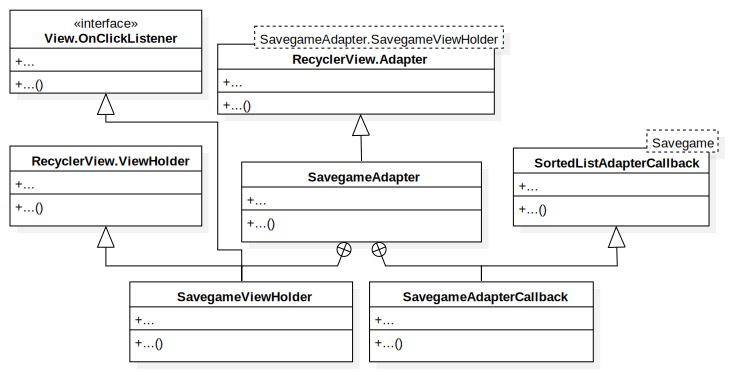
\includegraphics[width=1.0\textwidth]{resources/savegamestorage/SavegameAdapter}
	\caption{Spielstand SavegameAdapter}
\end{figure}

\subsection{Aufbau}
\subsectionauthor{\frank}

Wenn ein Spiel gespeichert oder geladen werden soll, geschieht dies durch einen
Aufruf der Instanz \code{SavegameStorage}. Um hier nicht mehrmals neuen Code,
welche alle Spiele gemeinsam haben, schreiben zu müssen, haben wir diese
Aufgabe an die Klasse \code{GameActivity} abgegeben. Da nun jedes Spiel von
\code{GameActivity} erben soll, müssen dadurch unter anderem zwei abstrakte
Methoden -- zum Speichern und Laden -- implementiert werden.
\code{onSaveGame(Bundle)} respektive \code{onLoadGame(Bundle)}. Diese Methoden
arbeiten jeweils mit einem \textbf{Bundle}, welchem die für einen
Speicherzustand nötigen Informationen übergeben beziehungsweise entnommen
werden können.

\begin{mdframed}[frametitle=Erklärung: Bundle]
Dies ist ein Objekt welches verschiedene Datentypen, wie zum Beispiel:
\emph{String, int} oder \emph{long}, mit \emph{String-Keys mapped} und hochperfomant
für \emph{Interprozesskommunikation} ist.
\end{mdframed}

 \unsure{Diesen Absatz eher in die Implementierung, oder?}
Das der Methode \code{onSaveGame} übergebene Bundle kann mit Methoden wie
\code{.putString} oder \code{.putStringArrayList} mit gefüttert werden.
Anschließend werden die gespeicherten Werte weiterverarbeitet und
abgespeichert. Das bedeutet, falls das Bundle unangetastet bleibt, kann
signalisiert werden, dass kein Speichern gewünscht ist, und so der Spielstand
nicht überschrieben wird. Dies ist sehr hilfreich, wenn ein Spiel gestartet,
der Zustand diesen aber nicht verändert wurde. So wird verhindert, dass die
Spielstandliste mit Startaufstellungen von Spielen überfüllt wird. Support für
das Löschen eines Spielstandes ist an dieser Stelle zum aktuellen Zeitpunkt
noch nicht vorhanden.

\let\thefootnote\relax\footnote{Ein Klassendiagramm der Spielstände, ist im Anhang zu finden.}
\chapter{Implementierung}

\section{Die Spieleverwaltung}
\sectionauthor{\frank}

Ziel eines derartigen Frameworks ist, dieses möglichst modular \unsure{Ist das
das Ziel?} zu entwickeln. Dazu gehört auch, es zu ermöglichen, Spiele einfach
und dynamisch hinzufügen zu können. Sicher könnte man dessen benötigten Klassen
erstellen und anschließend an irgendeiner Stelle in die App hardcoden. Doch wir
wollten all das, was zu diesem Prozess gehört, vereinfachen, und damit flüssiger,
angenehmer und vor allem modularer gestalten. Dadurch wird auch das
nachträgliche Ändern oder Löschen von Spielen trivial. Außerdem wird so der Weg
für zukünftige Automatisierung -- wie beispielsweise Spielständen -- geebnet.

\subsection{Deklaration von Spielen}

Die Deklaration und Deklaration von Spiele-Metadaten erfolgt strukturiert in
einer XML-Datei, \emph{games.xml}, welche durch eine \textbf{Document Type
Definition} (\textbf{DTD}) semantisch abgesichert ist. So wird gewährleistet,
dass die Spiele im passenden Format vorliegen, und so entsprechend
weiterverarbeitet werden können. Die Datei erlaubt außerdem die Zuordnung in
selbst gewählte Spiele-Kategorien, wie zum Beispiel \emph{Kartenspiele} oder
\emph{Brettspiele}.

Hier ist ein Auszug der Datei, welcher die verwendete DTD zeigt:

\begin{lstlisting}
<!DOCTYPE games [
    <!ELEMENT games (category*)>
    <!ELEMENT category (game*)>
    <!ATTLIST category id ID #REQUIRED>
    <!ATTLIST category title CDATA #REQUIRED>
    <!ATTLIST category icon CDATA #REQUIRED>
    <!ELEMENT game EMPTY>
    <!ATTLIST game title CDATA #REQUIRED>
    <!ATTLIST game description CDATA #REQUIRED>
    <!ATTLIST game icon CDATA #REQUIRED>
    <!ATTLIST game rules CDATA #REQUIRED>
    <!ATTLIST game tag CDATA #IMPLIED>
    <!ATTLIST game activity CDATA #REQUIRED>
]>
\end{lstlisting}

\subsubsection{Kategorien}

Wie man daraus ablesen kann, können unter dem Root-Element \code{games} beliebig
viele Kategorien hinzugefügt werden. Eine solche Kategorie wird beschrieben
durch drei verpflichtende Attribute. \code{id} ist eindeutig im gesamten
Deklarationsbereich, also der Datei zu wählen. Sie wird später weiter verwendet,
um eine Kategorie eindeutig identifizieren und wiederfinden zu können.
\code{title} ist die Bezeichnung dieser Kategorie. Hier ist es möglich, Text aus
der \emph{strings.xml}-Datei zu referenzieren. Solche Referenzierungen werden in
der Form \code{"@strings/ref"} angegeben, wobei \code{ref} für den
entsprechenden Identifikator steht. Außerdem ist noch ein Icon anzugeben, das
später beispielsweise im Navigation Drawer zu finden ist. Hier ist ebenfalls die
Referenzierung einer Resource möglich.

\subsubsection{Spiele}
\label{sssec:games}

Spiele werden analog unterhalb der Kategorien angegeben. Sie besitzen jedoch
unterschiedliche Attribute. \code{title} und \code{icon} stimmen mit der
Funktionalität deren einer Kategorie überein. Ihre Werte kann man
beispielsweise in der Spieleliste \improvement{Das in die Grundlagen} oder in
der Android-Actionbar sehen. Zusätzlich sind die beschreibenden Attribute
\code{description}, \code{rules} hinzuzufügen. Sie werden ebenfalls in
GUI-Elementen der App zu Finden sein. \code{activity} bestimmt später in der
laufenden Anwendung, welche Aktivität gestartet wird, wenn man auf das Spiel in
der Liste klickt. Die Aktivität muss im Package \emph{view} unter
\emph{activity} im Root-Package liegen, um gestartet werden zu können. Sie wird
mit ihrem Ort innerhalb dieses Paketes angegeben, zum Beispiel \emph{``Chess''}
Weitere Unter-Pakete sind möglich. Das letzte Attribut \code{tag} ist zur
genaueren Bestimmung der Eigenschaften eines Spiels gedacht und kann später in
der Aktivität des Spiel selbst abgefragt werden. Mit diesem Tag ist es denkbar,
weitere Varianten eines Spieles anzulegen, ohne dafür neue Aktivitäten
/ Klassen anfertigen zu müssen. Es besteht darüberhinaus die Möglichkeit,
mehrere Tags festzulegen; diese werden durch Verkettungszeichen | getrennt. Im
Falle eines 2-Spieler Schach-960's, lautet der Tag \code{``aiGame|chess960''}.

\subsubsection{Beispiel}

Die Datei mit genauer einer Kategorie und einem Spiel würde also so aussehen:

\begin{lstlisting}
<?xml version="1.0" encoding="utf-8"?>
<games>

    <category
        id="boardgames"
        title="@string/boardgames"
        icon="@drawable/icon_checkerboard">

        <game
            title="@string/game_chess_title"
            description="@string/game_chess_player_vs_ai"
            icon="@mipmap/ic_launcher"
            rules="@string/game_chess_rules"
            tag="aiGame"
            activity="Chess" />

    </category>

</games>
\end{lstlisting}

Die \textbf{DTD} wurde aus Platzgründen weggelassen.

\subsection{Die Spiele-Klasse}

Passend zu der Beschreibung eines Spiels in der XML-Datei gibt es die Klasse
\code{Game}. In ihr befinden sich die äquivalenten Attribute zu denen der
Markup-Datei. Außerdem besitzt diese Klasse eine Instanzmethode \code{boolean
isTaggedWith(String tag)}, welche abfragt, ob das übergebene Argument Teil des
Tags ist. So kann eine Spieleaktivität ganz ohne Umschweife die Eigenschaften
des zugehörigen Elements aus der Deklarationsdatei abfragen, um bestimmte
Abfolgen des Spielverlaufes zu verändern. Siehe \autoref{sssec:games}.

\subsection{Der Spielemanager}


\includegraphics{resources/tobecontinued}

\change{Bessere Graphik und Caption}
\begin{figure}[h]
	\centering
	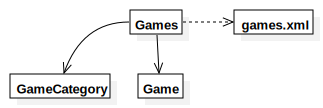
\includegraphics{resources/gamemanager/gamemanager_uml}
	\caption{Test}
	\label{fig:gm_uml}
\end{figure}

\section{Der Hub}
\sectionauthor{\leonard}

Der Hub besteht aus sehr vielen Teilen und hat auch viele Funktionen zu bieten.
Zum einen ist da der \textbf{Navigation Drawer}, welcher das Hauptmenü
darstellt. Des Weiteren sind da die \textbf{Fragments}, die Spielstände zum
Laden anbieten und alle Spiele, nach Kategorie aufgeteilt, anzeigen.

\subsection{Die Hub Activity}

Grundsätzlich arbeitet sie mit \emph{Tags}, welche bestimmen welches Fragment
gerade aktiv und zu sehen ist. Sie setzt den Titel der \textbf{Toolbar} passend
zu jedem Fragment. Außerdem wird hier der \emph{Navigation Drawer}
(kurz \emph{NavDrawer}) aufgebaut und gesteuert.

\subsubsection{Initialisierung}

\begin{lstlisting}[caption={Hub onCreate() Methode},captionpos=b]
private final char tagHub = '0', tagCards = '1', tagBoard = '2', tagInfo = '3', tagSettings = '4';
...
@Override
protected void onCreate(Bundle savedInstanceState) {
	super.onCreate(savedInstanceState);
	setDefaultValuesOfSettingsFirstTime();
	setContentView(R.layout.activity_hub);
	setupActionBar();

	drawer = (DrawerLayout) findViewById(R.id.drawer_layout);
	navigationView = (NavigationView) findViewById(R.id.nav_view);

	setupNavigationView();

	if (savedInstanceState == null) {
		currentTag = tagHub;
		loadHomeFragment();
	} else {
		setToolbarTitle();
	}
}
\end{lstlisting}

Die Methode in Zeile 39 setzt die Standardwerte der \emph{Einstellungen}, sie
wird nur aufgerufen wenn die App das erste mal startet. Weiter setzt
\code{setupActionBar()}, die \textbf{Toolbar} auf. Zeile 43 \& 44 weisen die
\textbf{Views} für den \emph{NavDrawer} zu und \code{setupNavigationView()}
definiert den \emph{NavDrawer} mit den jeweiligen Klick-Events. Die
\code{if(...)} Abfrage überprüft ob die App neu gestartet wurde und setzt
dementsprechend den \code{currentTag} auf \code{tagHub}, also dem Spielehub,
oder behält den momentanen und setzt den richtigen Titel für die
\textbf{Toolbar}. Die Variablen für die Tags werden als \code{final char}
zugewiesen, um nicht veränderbar zu sein.

\begin{lstlisting}[caption={Hub loadHomeFragment() Methode},captionpos=b]
private void loadHomeFragment() {
	selectNavMenu();
	setToolbarTitle();

	if (getSupportFragmentManager().findFragmentByTag(Character.toString(currentTag)) != null) {
		drawer.closeDrawers();
	return;
	}

	// add to the message queue
	new Handler().post(new Runnable() {
	@Override
	public void run() {
		Fragment fragment = getHomeFragment();
		FragmentTransaction fragmentTransaction = getSupportFragmentManager().beginTransaction();
		fragmentTransaction.setCustomAnimations(android.R.anim.fade_in, android.R.anim.fade_out);
		fragmentTransaction.replace(R.id.frame, fragment, Character.toString(currentTag));
		fragmentTransaction.commitAllowingStateLoss();
	}
});

drawer.closeDrawers();
}
\end{lstlisting}

Die Methode \code{loadHomeFragment} lädt das gewünschte \textbf{Fragment} in den
Vordergrund. \code{selectNavMenu()} markiert das ausgewählt \textbf{Fragment} im
\emph{NavDrawer}. Die \code{if(...)} Abfrage checkt ob das ausgewählte 
\textbf{Fragment} nicht schon im Vordergrund ist. Wenn es im Vordergrund ist,
wird der \emph{NavDrawer} einfach geschlossen. Ansonsten wird ein \code{Handler}
mit dem jeweiligen \textbf{Fragment} \emph{geposted}. Der \code{Handler} wird
mit einer \code{Runnable()} aufgerufen, welche Vorort implementiert wird. Mit
\code{getHomeFragment()} wird das \textbf{Fragment} geladen. Die Transaktion
bekommt eine eigene Animation zugewiesen und dann wird das zugehörige
\textbf{FrameLayout}, das \textbf{Fragment} und der \emph{Tag} deklariert. Diese
Herangehensweise mit einem \code{Handler} wird verwendet, da sie für größere
Datenmengen performanter ist. Am Ende wird der \emph{NavDrawer} geschlossen.

\begin{infobox}[frametitle=Handler]
Erlaubt das Senden und Ausführen von \textbf{Message} oder \textbf{Runnable}
Objekten in Verbindung mit der \textbf{MessageQueue} eines \emph{Threads}. Jeder
Handler ist einem \emph{Thread} und deren \textbf{MessageQueue} zugewiesen.
Kann zum Zeitversetzten ausführen eine Prozesses oder der Einreihung einer
Aktion für einen anderen \emph{Thread} benutzt werden.
\end{infobox}

\begin{lstlisting}[caption={Hub setupNavigationView() Methode},captionpos=b]
public void setupNavigationView() {
	navigationView.setNavigationItemSelectedListener(new NavigationView.OnNavigationItemSelectedListener() {
		@Override
		public boolean onNavigationItemSelected(@NonNull MenuItem menuItem) {
			char numericShortcut = menuItem.getNumericShortcut();
			switch (numericShortcut) {
				case tagHub:
				case tagCards:
				case tagBoard:
					currentTag = numericShortcut;
					break;
				case tagInfo:
					openPreferenceScreen(getString(R.string.nav_item_info), new InfoFragment());
					break;
				case tagSettings:
					openPreferenceScreen(getString(R.string.nav_item_settings), new SettingsFragment());
					break;
				default:
					currentTag = tagHub;
		}
	loadHomeFragment();
	return true;
	}
});
...
}
\end{lstlisting}

Hier werden dem \emph{NavDrawer} die Klick-Events zugewiesen. Die Abfrage
erfolgt durch den Vergleich des \code{currentTag} mit dem in der
\code{nav\_drawer\_items.xml} definierten \emph{NumericShortcut}.

\subsection{Die Fragments}

Die mit der Hub-Activity verbundenen Fragmente heißen \code{GameSelection} und
\code{Hub}. Ersteres ist für Brettspiele und Kartenspiele zuständig, zweiteres
für die Auflistung und Verwaltung laufender Spiele, also Spielstände.

\subsubsection{GameSelection}

Es ist möglich ein \textbf{Fragment} für mehrere Sachen zu Verwenden, auch können
sie von verschiedenen \emph{Activites} gerufen werden. Durch einen
\textbf{String}-Parameter in der Methode \code{newInctance(String)} wird
zwischen Brett- und Kartenspielen unterschieden.

\begin{lstlisting}[caption={Hub setupNavigationView() Methode},captionpos=b]
public static GameSelection newInstance(String category) {
	Bundle args = new Bundle();
	args.putString(EXTRA_CATEGORY, category);	
	GameSelection fragment = new GameSelection();
	fragment.setArguments(args);
	return fragment;
}

@Override
public void onCreate(@Nullable Bundle savedInstanceState) {
	super.onCreate(savedInstanceState);
	String gameCategory = getArguments().getString(EXTRA_CATEGORY);
	games = Games.getGameList(gameCategory);
}
\end{lstlisting}

In \code{onCreate(Bundle)} wird dann ermittelt, welches der beiden geladen wird.
Da der String in das \textbf{Bundle} des \textbf{Intent}s geladen wurde, kann
er so wieder heraus geholt werden. Die Methode \code{Game.getGameList{String}}
unterscheidet dann intern zwischen den beiden und gibt die entsprechende Liste
zurück.\\

\begin{lstlisting}[caption={GameSelection onCreateView() \& onActivityCreated() Methode},
captionpos=b]
@Nullable
@Override
public View onCreateView(LayoutInflater inflater, @Nullable ViewGroup container, @Nullable Bundle savedInstanceState) {
	return inflater.inflate(R.layout.fragment_game_selection, container, false);
}
@Override
public void onActivityCreated(@Nullable Bundle savedInstanceState) {
	super.onActivityCreated(savedInstanceState);
	View rootView = getView();
	if (rootView == null) {
		throw new NullPointerException("Root view is null");
	}
	RecyclerView recyclerView = (RecyclerView) rootView.findViewById(R.id.recyclerview_game_selection);
	RecyclerView.LayoutManager layoutManager = new LinearLayoutManager(getActivity());
	recyclerView.setLayoutManager(layoutManager);
	GameAdapter gameAdapter = new GameAdapter(games);
	recyclerView.setAdapter(gameAdapter);
}
\end{lstlisting}

In \code{onCreateView(...)} wird das \textbf{FrameLayout} zugewiesen. In
\code{onActivityCreated(...)} wird dann der \textbf{RecyclerView} und der
Adapter zugewiesen. Der Adapter ist diesem Fall der \code{GameAdapter}.

\begin{infobox}[frametitle=RecyclerView]
Ein flexibler \textbf{View}, welcher eine große Datenmenge in einem begrenzten
Fenster anzeigen kann. Dabei ist er sehr performant, da er schon genutzte
\textbf{View}s im \textbf{cache} platziert, um sie später wieder zu nutzen. 
\end{infobox}

\subsubsection{Spielehub}

Im Vergleich zu \code{GameSelection}, ist dieses Fragment etwas überfüllter, da
es viel mehr Funktionen hat. Zum einen wäre da der \textbf{FloatingActionButton}
(kurz FAB). Welcher zusätzlich zu der \emph{NavDrawer} Menüleiste, auch zu
Brett- und Kartenspielen weiter leiten kann. Hier speziell ist es sogar eine
\emph{nested} Version des \emph{FAB}s.

\begin{infobox}[frametitle=FloatingActionButton]
Ein runder Button der immer eine positive Aktion ausführt. Er
besitzt spezielle Bewegungsverhalten. Nested: Ein FAB welcher mehrere FABs
auftauchen lässt.
\end{infobox}

Die Methode \code{onCreateView(...)} fungiert wie bei \code{GameSelection}.

\begin{lstlisting}[caption={Spielehub onActivityCreated() Methode},captionpos=b]
@Override
public void onActivityCreated(@Nullable Bundle savedInstanceState) {
	super.onActivityCreated(savedInstanceState);
	View rootView = getView().getRootView();
	emptyText = (TextView) rootView.findViewById(R.id.fragment_hub_empty_textview);
	coordinatorLayout = (CoordinatorLayout) rootView.findViewById(R.id.coordinator_layout);
	setupAlphaAnimation();
	setupRecyclerView();
	checkSavegameAdapterCount();
	setupFabs(rootView);
}
\end{lstlisting}

Zunächst gibt es ein paar Zuweisungen von Variablen. In
\code{setupAlphaAnimation()} werden für den \code{emptyText} Animationen
gesetzt. Die Methode \code{setupRecyclerView()} weist den \textbf{RecyclerView}
und den \code{SavegameAdapter()} zu. Zudem wird hier noch ein
\textbf{ItemTouchHelper} initialisiert, welcher zum \textbf{RecyclerView}
gebunden wird und mit der inneren Klasse \code{GameSelectionCallback} aufgerufen
wird. Diese innere Klasse kümmert sich um das Löschen von Spielständen durch
wischen der Karten.

\begin{lstlisting}[caption={Spielehub setupRecyclerView() Methode},captionpos=b]
private void setupRecyclerView() {
	swipeRefreshLayout = (SwipeRefreshLayout) getView().findViewById(R.id.refresh_layout);
	recyclerView = (RecyclerView) getView().findViewById(R.id.recyclerview_game_selection);
	RecyclerView.LayoutManager layoutManager = new LinearLayoutManager(getActivity());
	recyclerView.setLayoutManager(layoutManager);
	
	setupAdapter();
	ItemTouchHelper itemTouchHelper = new ItemTouchHelper(new GameSelectionCallback());
	itemTouchHelper.attachToRecyclerView(recyclerView);

	recyclerView.addOnScrollListener(new RecyclerView.OnScrollListener() {
		@Override
		public void onScrolled(RecyclerView recyclerView, int dx, int dy) {
			if (dy > 0) {
				fabNewGame.hide();
			} else {
				fabNewGame.show();
			}
		}
	});
	swipeRefreshLayout.setOnRefreshListener(new SwipeRefreshLayout.OnRefreshListener() {
		@Override
		public void onRefresh() {
			alphaOut.setAnimationListener(new AnimationEndListener() {
				@Override
				public void onAnimationEnd(Animation animation) {
					setupAdapter();
					recyclerView.startAnimation(alphaIn);
					refreshComplete();
				}
			});
			recyclerView.startAnimation(alphaOut);
		}
	});
}
\end{lstlisting}

Des Weiteren werden ein \code{addOnScrollListener(...)} und ein
\code{setOnRefreshListener(...)} implementiert. Ersteres lässt den \emph{FAB}
beim runterscrollen verschwinden, damit auch der unterste Spielstand,
vollständig sichtbar ist. Zweiteres startet eine Aus- und Einblende-Animation
beim Aktualisieren des \textbf{RecyclerViews}, damit die Veränderung der Liste
flüssiger wirkt.

\subsection{Navigation Drawer}

Als Menü verwenden wir einen \emph{Navigation-Drawer}, welcher nur im \emph{Hub}
zur Verfügung steht und wie folgt aufgebaut ist.


\section{Chess}
\sectionauthor{\oliver}

Schach ist eines der bekanntesten und gleichzeitig eines der anspruchsvollsten
Spiele der Welt. Aufgrund der Komplexität und benötigten Weitsichtigkeit
schaffte es erstmalig erst 1996 der Schachcomputer "Deep Blue" von IBM den
damalig amtierenden Schachweltmeister Garro Kasparow zu besiegen.
\improvement{Beleg?} Heutzutage hingegen existieren viele Implementierungen
fähiger Schachprogramme und KI. In diesem Projekt wurde die Schachengine
\hyperlink{https://github.com/albertoruibal/carballo}{\emph{Carballo}}
verwendet. \unsure{Kommt das hier überhaupt hin? Wenn ja, mehr?} \info{Joa,
vielleicht etwas mehr Überleitung}

\subsection{Das Spielfeld}

Für das klassisch karierte Schachbrett wurde die Klasse
\code{CheckeredGameboardView} erstellt, welche wie der Name schon sagt von der
Android-Klasse \code{View} erbt. Hauptbestandteil ist ein zweidimensionales
Array aus Androids\code{Rect}, welche die einzelnen Felder des Spielfelds
darstellen. Diese werden nach Aufruf von \code{onSizeChanged} der Größe des
Displays angepasst und je nach Einstellung um die Stärke des gewünschten Randes
verschoben, sodass auf jedem Gerät ein identisches Spielerlebnis erzeugt werden
kann. Um bei einer Berührung auf die View zu ermitteln, auf welches der Felder
getippt wurde, setzt die Methode \code{getSquareFromTouch(int x, int y)} die in
\code{Rect} mitgelieferte Funktion \code{contains(int x, int y)} ein und gibt
die Array-Koordinaten des gesuchten Kästchens zurück. Bei der Kolorierung und
Markierung der Felder bezieht sich die Klasse auf die in den App-Einstellungen
festgelegten Werte.

\subsection{Der Chesswrapper}

In der Welt der Informatik sucht man den Begriff \emph{langlebig} vergeblich --
permanent werden Module und Codeabschnitte verändert und ausgetauscht. Auch bei
dieser Spielesammlung sind solche Modifikationen vorgekommen und werden wohl in
absehbarer Zeit wieder passieren. Aus diesem Grund ist die Schachlogik nur über
eine einzige Schnittstelle zugänglich, dem \code{ChessWrapper}. Dieser
umschließt alle benötigten Funktionen der verwendeten Schachbibliothek und
erleichtert das Austauschen der selbigen beachtlich. Neben grundlegenden
Funktionen, wie das Ausgeben der aktuellen Figurenaufstellung und das Setzen
von Schachzügen, beinhaltet der Wrapper auch die Funktionen der künstlichen
Intelligenz, welche sich in der gleichen Bibliothek befindet. In zukünftigen
Versionen werden diese Funktionen getrennt behandelt, um allgemein geltenden
Codemetriken gerecht zu werden.\unsure{Soll das so bleiben oder kommt das so
rüber als ob wir das schlecht gemacht haben?} \info{Was meinst du damit, es
wird getrennt behandelt? Haben wir da je darüber geredet?}

\subsection{Der MoveTranslator}
Schach besitzt ein ein Koordinatensystem, welches leider nicht mit dem 
Indexsystem eines Java-array übereinstimmt. Aus diesem Grund braucht man eine 
Hilfsklasse \code{MoveTranslator},welche in der Methode \code{numToString} aus 
einem Tupel von Integers einen String ausgibt, welcher von den 
\code{ChessWrapper} Methoden akzeptiert werden kann. Auf die selbe Art und Weise 
wandelt die Methode \code{stringToNum} aus einem String des Formats \emph{A4} 
einen Tuple um, welcher Array-kompatible Koordinaten besitzt. Hierfür verwenden 
die privaten Methoden \code{colToChar},\code{rowToChar},\code{charToCol}, und 
\code{charToRow} die eigenschaft von Chars und Integern, mittels der \emph{+} 
und \emph{-} Operatoren miteineander addiert und subtrahiert zu werden.


\subsection{Die Chess Activity}

In der Activity Chess werden die oben genannten Komponenten unter einem Dach 
vereint und miteinander kombiniert.

\subsubsection{onLoadGame()}

Die Methode \code{onLoadGame()},welche die abstrakte Methode der Oberklasse
\code{GameActivity} überschreibt wird sowohl bei neuen Spielen, als auch beim
Laden eines alten Spielstandes aufgerufen und setzt in Kenntnis, um welche Art
von Schachspiel es sich handelt. Dies gelingt durch das überprüfen der gesetzten
Tags in der Instanz von \code{Game()}, welche ebenfalls über \code{GameActivity}
vererbt wurde. Die hierbei infrage kommenden Tags sind \emph{aiGame}, welches
anzeigt ob es sich um ein Mensch gegen Computer Spiel handelt und
\emph{chess960}, welcher definiert, ob die erweiterten Schachspielregeln für
Chess960 verwendet werden, dazu später mehr.\newline Im selben Vorgang wir eine
Instanz des \code{Chesswrapper} erstellt, welcher die Spiellogik und eine
unberührte Spielaufstellung beinhaltet. Falls ein alter Spielstand geladen wird,
wird bei \code{onLoadGame()} zusätzlich ein Bundle übergeben, welches die
bisherigen Spielzüge beinhaltet. Diese werden dem Chesswrapper mithilfe der
Methode \code{doMoves()} übergeben, sodass dieser seine Figurenaufstellung auf
den aktuellen Stand bringen kann. Auch der \code{ChessHistoryAdapter} wir hier
mit den bereits getätigten Zügen aufgefüllt.

\subsubsection{onCreate()}
In der \code{onCreate()} wird das Spiel für die eigentliche Benutzung 
vorbereitet. So werden das \code{FrameLayout} und \code{CheckeredGameboardView} 
aus der \code{chess.xml} geladen und referenziert. Ein zweidimensionales Array 
der Klasse \code{ImageView} stellt die Spielfiguren dar, wobei darauf geachtet 
werden muss das es die selbe Große besitzt wie das Spielfeld. In 
\code{setFieldFromFEN} wird dieses Array mit den Figuren das aktuellen 
Spielfelds überschrieben, wobei der \code{ChessWrapper} die nötigen Daten 
mittels eines FEN-Strings liefert. Die Methode \code{addImages()}, welche die 
korrekten Größen und Koordinaten der Bilder festlegt darf allerdings erst 
aufgerufen werden nachdem das Layout des Spielfeldes gesetzt wurde, da sich eine 
Imageview auf die Große des darunterliegenden \code{Rect} bezieht, welches zuvor 
noch nicht gesetzt wäre. Mithilfe des \code{ViewTreeObserver} welcher den 
Listener \code{addOnGlobalLayoutListener()} zur Verfügung stellt kann dieses 
Problem einfach gelöst werden. Für die weitere Verwendung kann 
\code{addImages()} problemlos verwendet werden, da sich das Layout von nun an 
nicht ändert. Mit \code{ setupRecyclerView()} wird die RecyclerView mit eigens 
geschriebenen Adaptern aufgesetzt\newline
Damit man die Spielfelder später auch antippen kann wird letztendlich der 
\code{CheckeredGameboardView} ein \code{OnTouchListener} angelegt, welcher bei 
einem Touch-Event das entsprechende Kästchen des Spielfeldes als Tuple-paar an 
die Methode \code{onSquareClicked()} übergibt.

\subsubsection{setFieldFromFEN()}

Die Methode \code{setFieldFromFEN()} dient zur Neubelegung des zweidimensionalen 
Imageview-Arrays, welches die Spielfiguren beinhaltet. Zu Anfang der 
Neubesetzung werden erst alle Einträge aus dem Array gelöscht, um eventuelle 
Fehler zu vermeiden. Darauf wird der FEN-String geparst, während ein X und ein Y 
Wert dementsprechend hoch zählen. Der Notation entsprechend wird bei einem 
\emph{/} eine neue Schachzeile angefangen, sodass der Y-Wert erhöht wird, und 
der x-Wert auf 0 zurück gesetzt wird. Im Falle einer Zahl, welche leere Felder 
anzeigt, wird der X-Wert um die entsprechende Zahl erhöht. Falls der String 
jedoch einen Buchstaben als nächstes hat, wird and die entsprechende Koordinate 
eine neue Imageview erstellt, dessen Ressource man anhand der fest codierten Map 
und dem ausgelesenem Buchstaben heraussuchen kann.

\subsubsection{onSquareClicked()}

Die Methode \code{onSquarClicked()} ist das Herzstück der Chess Activity und
besitzt die komplette Logik welche die Züge des Spielers verwaltet. Sie bekommt
vom \code{OnTouchListener} des Spielfedes die Koordinaten des Feldes zurrück auf
welches gerade getippt wurde. Ob dieses Tupel nun eine Auswirkung auf das Spiel
hat hängt von einer Vielzahl von Eigenschaften ab, welche elegant mit boolescher
Algebra kombiniert werden können. Falls man zuvor noch nicht auf ein Feld
getippt hat und nun eine valide Auswahl getroffen hat, wird dieses Feld nun in
der Klasse als \code{logged} gespeichert, sodass bei nochmaligem Tippen auf ein
anderes Feld geprüft werden kann, ob ein gültiger Schachzug von \code{logged}
zum neuen Feld durchgeführt werden kann. In diesem Fall muss zuerst der
Spezialfall der Promotion getestet werden, bei welcher der Promotionsdialog
geöffnet wird, dazu später mehr. Im Regulärfall wird der Zug durch
\code{animatefigure()} durchgeführt, was ebenfalls eine Animation der Figur zur
Folge hat. Falls es sich um ein Spiel gegen die künstliche Intelligenz handelt
wird nun auch ein Zug der KI berechnet und ausgeführt.

\subsubsection{promotionDialog()}
Der \code{promotionDialog} wird im dem Spezialfall aufgerufen, in welchem ein 
Bauer die letzte Zeile der gegenüberliegenden Seite betritt. Wenn dies als 
normaler Spielzug übergeben wird setzt die Schachlogik automatisch eine Dame als 
gewählte Promotionsfigur. Dies ist zwar in den meisten fällen die beste Wahl, 
dennoch kann diese Entscheidung das Spiel zu Gunsten des Gegners fallen, z.B. 
wenn dadurch ein Patt ausgelöst wird, welches man durch eine Übermacht an 
Figuren zu einem Schachmatt ausbauen könnte. Ebenfalls kann es in sehr seltenen 
Fällen vorkommen, das ein Springer, welcher andere Angriffsmöglichkeiten als die 
Dame hat als neue Figur zu einem sofortigen Gewinn des Spieles führen könnte. 
Deswegen muss man auswählen können, welche der Vier Figuren Dame, Läufer, Turm 
und Springer man als Promotionsfigur wählt. Dies wird durch einen Alterdialog 
realisiert, welcher Vier Imageviews für die entsprechenden Figuren besitzt, jede 
von ihnen mit einem eigenen \code{PromotionClickListener}, welcher den Dialog 
beendet und den entsprechenden  \code{promotionmove} mit der jeweiligen neuen 
Figur durchführt.


\section{Kartenspiele}
\sectionauthor{\philipp}

Wir implementierten drei Kartenspiele in unsere Applikation: Mau-Mau,
Bauernkrieg und Offiziersschafkopf (auch: Aufgelegter Schafkopf). Letzteres ist
für 2 Spieler ausgelegt und vor allem in Bayern bekannt. Trotz der relativ
komplexen Art in Schafkopf Stiche zu erzielen, war uns die JDroid Bibliothek
eine große Hilfe. Diese Bibliothek brachte auch Mau-Mau und Bauernkrieg bereits
mit, welche beide lediglich abgeändert werden mussten.  Aus diesem Grund
fokussieren wir uns in diesem Teil auf Schafkopf, zumal in diesem Spiel alles
verwendet wird, was auch in den anderen beiden verwendet wird. Jedem Spiel ist
ein Menu mit \emph{Start} Knopf vorgeschalten, in welchem man die Regeln
nochmals lesen könnte.

\subsection{Ranks und Suits}

Zum weiteren Verständnis zeige ich hier die in Schafkopf genutzten enums auf,
auf denen das Deck basiert.

\begin{lstlisting}[caption={Enums für Kartenwertigkeiten},captionpos=b]
public enum Suit
{
    EICHEL, GRUEN, HERZ, SCHELLEN
}
public enum Rank
{
    ASS, OBER, UNTER, ZEHN, KOENIG, NEUN, ACHT, SIEBEN
}
\end{lstlisting}

\subsection{Schafkopf Board}

Wir nutzen zwei Klassen für das Schafkopf Spiel: \code{schafkopf} und
\code{initiateGame}. \code{schafkopf} erbt von \code{CardGame}, einer
Bibliotheksklasse, welche alle wichtigen Methoden von JDroid implementiert. Bei
Erzeugen der Schafkopf Klasse wird das Board erstellt und in \code{main()}
zunächst das Deck und ein initiateGame Objekt auf dessen Basis.
\code{InitiateGame} initialisiert alle nötigen Hände; sprich Bids, Stacks und
Hands, und weist ihnen Locations zu. Ist dies abgeschlossen, wird
\code{initPlayers()} und \code{setPlayerMove()} aufgerufen, um fortzufahren.

\begin{lstlisting}[caption={Beispiel Hands initialisieren},captionpos=b]
private final Location[] handLocations =
        {
            new Location(100, 850),//spieler1
            new Location(200, 850),

            new Location(100, 100),//spieler2
            new Location(200, 100),
        };

public void setHand(){
    hands = deck.dealingOut(16, 2, true);
    StackLayout[] layouts = new StackLayout[16];

    for (int i = 0; i < 16; i++)
    {
        layouts[i] = new StackLayout(handLocations[i]);
        hands[i].setView(board, layouts[i]);
        hands[i].setTargetArea(new TargetArea(bidLocations[0]));
        if(i>8)hands[i].setTargetArea(new TargetArea(bidLocations[1]));
        hands[i].draw();
    }

    board.hands = this.hands;
}

\end{lstlisting}

\subsection{initPlayers()}

Diese Methode ist das Herzstück unserer Kartenspiele. Hat derjenige Spieler,
welcher eben an der Reihe ist, eine Karte ausgewählt und auf den Bid
transferiert, dann gibt es nun zwei Möglichkeiten:

\begin{itemize}
	\item 1. Auf beiden Bids befinden sich Karten und der Stich wird ausgewertet
	\item 2. Auf nur einem Bid befindet sich eine Karte, \code{setPlayermove(otherPlayer)} wird 		 aufgerufen
\end{itemize}

Im ersten Falle wird \code{sticht()} aufgerufen und getestet, wer den Stich
macht. Die Karten werden auf den Stack des Gewinners transferiert, es wird
getestet, ob das Spiel vorbei ist, und die Kartenzahl wird aktualisiert.
Zuletzt wird noch der \code{Playermove} auf den Gewinner gesetzt und er darf
wieder eine Karte ausspielen.

\begin{lstlisting}[caption={initPlayers gamecycle},captionpos=b]
if (isBidFull()) {
    if (sticht(0) == 0)
    {
        delay(2000);
        transferBidsToStock(0);
        delay(1500);
        if(isGameOver())
        calculateResult();

        setPlayerMove(0);
    }

    else {
        delay(2000);
        transferBidsToStock(1);
        delay(1500);
        if(isGameOver())
        calculateResult();

        setPlayerMove(1);
    }
}
else setPlayerMove(1);
\end{lstlisting}

\subsection{Berechnung der Stiche}

Stiche berechnen ist im Schafkopf eine relativ komplexe Angelegenheit, da es
viele verschiedenen Trümpfe gibt. Das Ganze wird in der Methode
\code{sticht(int Player)} abgehandelt. Der Methode wird der Spieler, der gerade
die erste Karte angespielt hat, als Integer mitgegeben. Zunächst wird getestet,
ob der Spieler Trumpf angespielt hat mit \code{isTrumpf(int Player)}. Das wird
festgestellt, indem man testet, ob die Karte auf dem bid entweder ein Ober,
Unter oder Herz ist.

\begin{lstlisting}[caption={isTrumpf Methode},captionpos=b]
public boolean isTrumpf(int Player) {
    // int Player = Player der ausspielt
    if (bids[Player].getLast().getRank() == Rank.OBER
            || bids[Player].getLast().getRank() == Rank.UNTER
            || bids[Player].getLast().getSuit() == Suit.HERZ)
    {
        return true;
    }
    return false;
}
\end{lstlisting}

Ist diese Karte Trumpf, muss geprüft werden, ob der Trumpf höher ist.

\code{isTrumpfHigher(int Player)}: 

Player = Spieler, der ausspielt

Der Ablauf ist folgender:
\begin{lstlisting}[caption={isTrumpfHigher Methode},captionpos=b]
public boolean isTrumpfHigher(int Player) {
    int otherPlayer = (Player + 1) % 2
        if (isOber(Player))
        {
            if (isOber(otherPlayer))
            {
                if (isColorHigher(otherPlayer))
                    return false;
            }
            return true;
        }

        else if(isUnter(Player))
        {
            if (isOber(otherPlayer))
                return false;

            if (isUnter(otherPlayer))
            {
                if (isColorHigher(otherPlayer))
                    return false;
            }
            return true;
        }

        else if(isHerz(Player))
        {
            if (isOber(otherPlayer))
                return false;

            if (isUnter(otherPlayer))
                return false;

            else if (isHerz(otherPlayer))
            {
                if (isRankHigher(otherPlayer))
                    return false;
            }
            return true;
        }

    return false;
}
\end{lstlisting}
 
\code{isRankHigher()} und \code{isColorHigher()} funktionieren auf ähnliche
Weise: man überprüft welche Karten ID höher beziehungsweise niedriger ist. Den
Suits und Ranks werden jeweils IDs zugewiesen, in der Reihenfolge, wie sie in
den enums angegeben sind.

\begin{lstlisting}[caption={IDs am Beispiel von isColorHigher},captionpos=b]
public boolean isColorHigher(int Player)
{
    int otherPlayer = (Player + 1) % 2;

    if(bids[Player].getLast().getSuitId() < bids[otherPlayer].getLast().getSuitId())
    {
        return true;
    }
    return false;
}
\end{lstlisting}

Ist die gespielte Karte kein Trumpf, dann wird geschaut, ob die Karten dieselbe
Farbe habe. Wenn dem so ist und die Karte des anderen Spielers außerdem eine
Trumpfkarte ist, gewinnt dieser Spieler den Stich. Wenn nicht, wird
\code{isRankHigher()} aufgerufen und derjenige mit dem höheren Rang gewinnt.

Sind diese Aufrufe alle abgearbeitet, dann wird getestet ob nur der Spieler
Trumpf ausgespielt hat, der die zweite Karte gelegt hat. Wenn ja gewinnt er,
wenn nicht der andere Spieler.

Zuletzt wird getestet, ob beide Karten nicht dieselbe Farbe haben, sprich eine
Karte liegt. Spieler zwei muss nicht bekennen, und darf legen was er will. Dann
gewinnt Spieler 2.

Trifft keine der if - Abfragen zu, bekommt automatisch der Spieler, der
ausspielt, den Stich.

Alles in allem sieht die ganze Methode folgendermaßen aus:

\begin{lstlisting}[caption={sticht() Methode},captionpos=b]
public int sticht(int Player)
{
    int otherPlayer = (Player + 1) % 2;

    if(isTrumpf(Player))
    {
        if (isTrumpfHigher(Player))
            return Player;
        return otherPlayer;
    }
    if(sameColor()) {
        if (isTrumpf(otherPlayer)) return otherPlayer;
        if (isRankHigher(Player)) return Player;
            else return otherPlayer;
    }
    if(isTrumpf(otherPlayer))return otherPlayer;
    if(!sameColor()) return otherPlayer;
    return Player;
}
\end{lstlisting}

Das Ende einer jeden Stechen Phase ist das transferieren der Karten und
Weitergeben des aktiven Spielers.

\begin{lstlisting}[caption={TransferBidsToStock und setPlayerMove},captionpos=b]
private void transferBidsToStock(int playerWon)
{
    bids[0].setTargetArea(new TargetArea(stackLocations[playerWon]));
    bids[1].setTargetArea(new TargetArea(stackLocations[playerWon]));
    bids[0].transferNonBlocking(bids[0].getLast(), stacks[playerWon], true);
    bids[1].transferNonBlocking(bids[1].getLast(), stacks[playerWon], true);
}

private void setPlayerMove(int playerWon)
{
    if(playerWon==0)
    {
        if(isGameOver())
            calculateResult();

        for (int i = 0; i < 8; i++) hands[i].setTouchEnabled(true);
        for (int i = 8; i < 16; i++) hands[i].setTouchEnabled(false);
    }
    if(playerWon==1)
    {
        if(isGameOver())
            calculateResult();

        for (int i = 0; i < 8; i++) hands[i].setTouchEnabled(false);
        for (int i = 8; i < 16; i++) hands[i].setTouchEnabled(true);
    }
}
\end{lstlisting}

Um Karten zu transferieren, muss man dem bid einfach ein neues Ziel zuweisen und
es wird, mitsamt der durch die Bibliothek mitgebrachten Animation, transferiert.

Beim Spieler, der nun am Zug sein wird, wird \code{setTouchEnabled()} auf true
gesetzt, beim anderen auf false.

\subsection{GameOver}

Das Spiel ist vorbei, wenn alle 32 Karten auf den stacks liegen. Dazu wird nach
jedem Stich getestet, ob die Anzahl aller Karten auf den Stacks 32 ergeben.

\begin{lstlisting}[caption={isGameOver() Methode},captionpos=b]
private boolean isGameOver(){
    if(stacks[0].getNumberOfCards() + stacks[1].getNumberOfCards() == 32)
        return true;
    return false;
}
\end{lstlisting}

Die Punktzahl wird in \code{calculateResult()} berechnet. Dort werden die Anzahl
der in den Stacks vorhandenen Assen, Königen, und so weiter multipliziert mit
deren Wertigkeiten zusammengerechnet. Um dies anzuzeigen, gibt \code{calculate}
die Punktzahl an \code{winLabel(int[] points)} weiter. \code{WinLabel} erzeugt
\code{Textactors} mit den Strings \emph{GEWONNEN} und \emph{VERLOREN} und den
Punktzahlen.

\section{Die Spielstände}
\sectionauthor{\leonard}

Wie schon in der Architektur beschrieben, werden für die Spielstände die Klassen
\code{SavegameStorage}, \code{Savegame} und \code{SavegameAdapter} benutzt. Im
Folgenden wird näher auf diese Klassen eingegangen.

\subsection{SavegameStorage}

ist in einem Singleton-Pattern geschrieben. Gründe dafür sind einerseits, dass
der Speicher nur von einer Instanz aufgerufen werden soll, damit keine Speicher-
oder Ladefehler entstehen. Andererseits ist es wichtig, zu kontrollieren, wann
und wie auf den Speicher zugegriffen wird.

\begin{lstlisting}[caption={SavegameStorage Singleton},captionpos=b]
public static SavegameStorage getInstance() {
	if (instance == null) {
		synchronized (SavegameStorage.class) {
			if (instance == null) {
				instance = new SavegameStorage();
			}
		}
	}
	return instance;
}
\end{lstlisting}

\code{synchronized} wird hier verwendet um das Pattern \emph{Thread-Sicher} zu
machen.

\subsubsection{Der Speicherungsvorgang}

erfolgt durch die Nutzung von \textbf{SharedPreferences} (kurz SharedPref) in
Android.

\begin{infobox}[frametitle=SharedPreferences]
Ein Interface welches das Speichern und Laden von \emph{Key-Value} Paaren auf
dem Android Gerät ermöglicht. Modifikation von SharedPref müssen durch einen
SharedPref Editor geschehen.
\end{infobox}
Zur Laufzeit werden alle Spielstände als \code{ArrayList<Savegame>} gehandhabt.
Sobald etwas gespeichert werden soll, wird die Liste dementsprechend geändert und
durch \textbf{Gson} in \textbf{JSON} serialisiert und per
\textbf{SharedPreferences} unter einem \emph{Key} als String gespeichert. Beim
Laden erfolgt der Aufruf des \textbf{JSON}-Strings wieder durch den selben
\emph{Key} wie beim Speichern. Anschließend wird der String deserialisiert und
wieder in seine ursprüngliche Form, einer \code{ArrayList<Savegame>}, gebracht.

\begin{lstlisting}[caption={SavegameStorage Konstruktor},captionpos=b]
private SavegameStorage() {
	saveGameList = new ArrayList<>();
	savegamesSharedP = App.getContext().getSharedPreferences(SAVE_DATA_NAME, Context.MODE_PRIVATE);
	String saveGameListAsString = savegamesSharedP.getString(SAVE_DATA_KEY, "");
	if (!saveGameListAsString.isEmpty()) {
		saveGameList = gson.fromJson(saveGameListAsString, gsonType);
	}
}
\end{lstlisting}

In Zeile 216 sieht man die Zuweisung der \textbf{SharedPreferences} Variable
durch die Methode \code{getSharedPreferences(..., ...)}, welche als erstes
Argument den Dateinamen enthält und als zweites einen Zugriffsmodus, welcher in
diesem Fall der \emph{MODE\_PRIVATE} ist. Dieser Modus verhindert den Zugriff
anderer Apps auf die gespeicherten Daten.\\ Weiter erkennt man das Laden des
\textbf{JSON}-Strings durch \code{savegamesSharedP.getString(Key, Defaultwert)}.
Wenn dieser String dann etwas beinhaltet, dann wird er deserialisiert und
zugewiesen, ansonsten wird mit einer leeren Liste gearbeitet.

\begin{lstlisting}[caption={SavegameStorage Speicherfunktionen},captionpos=b]
public synchronized void addSavegame(Savegame savegame) {
	if (savegame != null) {
		saveGameList.add(savegame);
		putStringToEditor();
	}
}

public synchronized void updateSavegame(Savegame savegame) {...}

public synchronized void deleteSavegame(Savegame savegame) {...}

private synchronized void putStringToEditor() {
	for (Savegame savegame : saveGameList) {
		savegame.bundle.setClassLoader(null);
	}
	String saveGameListToString = gson.toJson(saveGameList, gsonType);
	SharedPreferences.Editor editor = savegamesSharedP.edit();
	editor.putString(SAVE_DATA_KEY, saveGameListToString);
	editor.apply();
}
\end{lstlisting}
 
Ob \emph{add-()}, \emph{update-()} oder \emph{deleteSavegame()}; alle diese
Methoden arbeiten gleich. Sie bekommen ein Savegame als Parameter und verändern
damit die interne \code{saveGameList}. Am Ende wird diese mit
\code{putStringToEditor()} via \textbf{Gson} serialisiert und dann mit
\textbf{SharedPreferences} gespeichert.

\begin{lstlisting}[caption={SavegameStorage Suche der Spielstände},captionpos=b]
public synchronized Savegame getFromUuid(String uuid) {
	if (uuid != null) {
		for (Savegame savegame : saveGameList) {
			if (savegame.uuid.equals(uuid)) {
				return savegame;
			}
		}
	}
	return null;
}
\end{lstlisting}

Eine sehr einfache, dennoch essentielle Methode ist die \code{getFromUuid()},
welche das zu einer \code{UUID} zugehörige \code{Savegame} zurückgibt.

\subsection{Savegame}

Das ist die \emph{Objekt-Klasse}, welche einen Spielstand darstellt. Sie besteht
aus 4 wesentlichen Variablen und wird wie folgt aufgebaut:

\begin{lstlisting}[caption={Savegame Variablen \& Konstruktor},captionpos=b]
public String uuid; public String gameUuid; public Bundle bundle; public Date
date;

public Savegame(String gameUuid, Bundle bundle) {
	this.uuid = UUID.randomUUID().toString();
	this.gameUuid = gameUuid;
	this.bundle = bundle;
	this.date = new Date();
}
\end{lstlisting}

Jeder Spielstand ist durch eine \code{UUID} eindeutig identifizierbar und somit
einzigartig. Diese wird beim Anlegen eines neuen Spielstandes generiert.  Die
\code{gameUuid} wird dem \emph{Konstruktor} übergeben und identifiziert den
Spielstand mit dem zugehörigen Spiel aus \code{games.xml}.  Das \code{Bundle}
enthält alle spielspezifischen Informationen die wichtig sind, sie werden vom
jeweiligen Spieleentwickler selbst gewählt. Das Datum dient der Anzeige und
Sortierung der Spielstände im Startbildschirm (\code{Hub}) und wird bei jeder
Aktualisierung erneuert.\\ Außerdem implementiert \code{Savegame} das Interface
\code{Comparable<Savegame>} und überschreibt die \code{equals()}-Methode damit
\code{SavegameAdapter} diese zum Sortieren benutzen kann.

\begin{lstlisting}[caption={Savegame compareTo() \& equals()},captionpos=b]
@Override
public boolean equals(Object obj) {
	return obj instanceof Savegame && this == obj;
}

@Override
public int compareTo(@NonNull Savegame o) {
	return date.compareTo(o.date);
}
\end{lstlisting}

Weitere Methoden, die \code{Savegame} besitzt, sind die \code{update()} und die
\code{getDateString()}-Methode. Wobei erstere, wie der Name schon sagt, für das
Aktualisieren des \code{Savegame}-Objektes zuständig ist, und zweiteres dafür
sorgt, dass \code{SavegameAdapter} das Datum in Textform darstellen kann.

\begin{lstlisting}[caption={Savegame update() \& getDateString()},captionpos=b]
public void update(Bundle bundle) {
	this.bundle = bundle;
	this.date = new Date();
}

public String getDateString() {
	String str;
	Locale locale = Locale.getDefault();
	if (DateUtils.isToday(date)) {
		str = SimpleDateFormat.getTimeInstance(SimpleDateFormat.SHORT, locale).format(date);
	} else if (DateUtils.isYesterday(date)) {
		str = App.getContext().getString(R.string.yesterday);
	} else if (DateUtils.isLastWeek(date)) {
		str = DateUtils.dateToCalendar(date).getDisplayName(Calendar.DAY_OF_WEEK, Calendar.LONG, locale);
	} else {
		str = SimpleDateFormat.getDateInstance(SimpleDateFormat.SHORT, locale).format(date);
	}
	return str;
}
\end{lstlisting}

\subsection{SavegameAdapter}

Diese Klasse erstellt für den Startbildschirm (\code{fragment.Hub}) Karten, die
genutzt werden um Spielstände in einem \code{RecyclerView} anzuzeigen und zu
laden. Außerdem weist sie die Klick-Events zu und sortiert die Spielstände nach
dem Datum.

Im \emph{Konstruktor} holt sich die Klasse die Spielstände von
\code{Savegamestorage} und führt sie intern als \textbf{SortedList<Savegame>}.
Wegen dieser \textbf{SortedList} wird die innere Klasse
\code{SavegameAdapterCallback} implementiert. Diese erbt von
\code{SortedListAdapterCallback<>} und hat den Zweck, die Liste mit
\textbf{RecyclerView.Adapter} zu binden. So ist es möglich die Liste zu
sortieren und aktuell zu halten.

Wenn die Klasse gerufen wird oder eine Aktualisierung verlangt wird, kümmert
sich \code{onBindViewHolder(ViewHolder, Position)} darum, dass alle
Spielstände jeweils einer Karte zugeordnet werden.

\begin{lstlisting}[caption={SavegameAdapter onBindViewHolder() Methode},captionpos=b]
@Override
public void onBindViewHolder(SavegameViewHolder holder, int position) {
	Savegame savegame = mSavegames.get(position);
	Game game = Games.getFromUuid(savegame.gameUuid);
	if (game != null) {
		holder.gameTitle.setText(game.getGameTitle());
		holder.gameSubtitle.setText(game.getGameDescription());
		holder.gameIcon.setImageDrawable(App.getContext().getDrawable(game.getGameIconId()));
		holder.gameDate.setText(savegame.getDateString().toUpperCase());
	}
}
\end{lstlisting}

\code{onBindViewHolder(...,...)} hat als erstes Argument den \textbf{ViewHolder}.
Dieser ist als innere Klasse implementiert und schaut wie folgt aus:

\begin{lstlisting}[caption={SavegameAdapter SavegameViewHolder Klasse},captionpos=b]
class SavegameViewHolder extends RecyclerView.ViewHolder implements View.OnClickListener {

	private final String ACTIVITY_PACKAGE = ".view.activity.";
	private final ImageView gameIcon;
	private final TextView gameTitle, gameSubtitle, gameDate;

	SavegameViewHolder(View itemView) {
		super(itemView);
		gameIcon = (ImageView) itemView.findViewById(R.id.icon_savegame);
		gameTitle = (TextView) itemView.findViewById(R.id.text_game_title);
		gameSubtitle = (TextView) itemView.findViewById(R.id.text_game_subtitle);
		gameDate = (TextView) itemView.findViewById(R.id.text_date);
		itemView.setOnClickListener(this);
	}

	@Override
	public void onClick(View v) {...}
}
\end{lstlisting}

Der \emph{Konstruktor} weist die \textbf{View}s zu und setzt diese auf einen
\textbf{OnClickListener}. Jener ist mit der Methode \code{onClick(View)}
implementiert und gibt den jeweiligen Karten die richtigen \textbf{Intent}s zu
den \textbf{Activities}.\\

\begin{lstlisting}[caption={SavegameAdapter Grundlegende Methoden},captionpos=b]
@Override
public int getItemCount() {
	return mSavegames.size();
}

public void addItem(Savegame savegame) {
	mSavegames.add(savegame);
	savegameStorage.addSavegame(savegame);
}

public void removeItem(int position) {
	Savegame savegame = mSavegames.removeItemAt(position);
	savegameStorage.deleteSavegame(savegame);
}

public Savegame get(int position) {
	return mSavegames.get(position);
}
\end{lstlisting}

Grundlegende Methoden wie \code{getItemCount()},
\code{add-  \& removeItem(Savegame)} oder \code{get(Position)} sind auch in
\code{SavegameAdapter} enthalten. Wobei \code{add \& remove} auf
\code{SavegameStorage} zugreifen, um dem Nutzer die Möglichkeit zu bieten,
seine Spielstände zu löschen. Diese Funktion wird in \code{fragment.Hub}
realisiert.

\chapter{Evaluierung}

\section{Schach}
\sectionauthor{\frank}

Im Folgenden soll der Schachteil unserer Applikation evaluiert werden. Zum
aktuellen Stand sieht der Bildschirm des Schachspiels folgendermaßen aus,
\autoref{fig:screen}. Man sieht im großen Mittelteil das Spielbrett mit den
Schachfiguren darauf. Man erkennt, dass Weiß sich im Schachmatt befindet anhand
der \textbf{Snackbar} am unteren Bildschirmrand.

\begin{infobox}[frametitle=Snackbar]
Die von Android mit der API-Version eingeführte Snackbar ermöglicht es,
zeitlich begrenzte Nachrichten am unteren Ende eines Layouts, meist des
gesamten Bildschirms, einzublenden. Der Snackbar kann ein Knopf und eine
Wisch-Funktion hinzugefügt werden, welche man im Code mit Aktionen verbinden
kann, die danach ausgeführt werden. Wie beispielsweise ein \emph{Undo}-Knopf,
der das Löschen einer Nachricht rückgängig machen lässt.
\end{infobox}

Zwischen der Snackbar und dem Spielfeld kann man die Schachhistorie erkennen,
worin man die letzten Versuche von Weiß sieht, sich aus dem sicheren Ende zu
befreien. Der obere Bildschirmrand zeigt den Titel des Spiels und rechts ist der
Knopf, über den man auf die Spielregeln kommt. Das bedeutet also
zusammengefasst: Die Schachoberfläche sieht genauso aus, wie sie es sollte.

\subsubsection{Demonstration}

Um die Funktionalität des Schachspiels zu beweisen, haben wir uns eine besondere
Schachaufstellung herausgesucht:

\code{7k/P1Q5/8/3pP3/3P4/8/1R6/R3K3 w Q d6 97} siehe \autoref{ssec:fen}

Die grafische Darstellung dieser Aufstellung kann man in \autoref{fig:special}
sehen. Das besondere an diesen Positionen ist, dass man die meisten Sonderzüge
eines Schachspiels daran demonstrieren kann:

\begin{itemize}
	\item Normaler Zug
	\item Schachmatt
	\item Patt
	\item Remis durch 50-Züge-Regel
	\item Rochade
	\item En passant
	\item Promotion
	\item (Schach-)Matt durch Promotion
\end{itemize}

\subsubsection{Normaler Zug}

Da ein normaler Zug jeden der folgenden Züge betrifft, wird er an dieser Stelle
nicht weiter erläutert.

\subsubsection{Schachmatt}
\label{sssec:checkmate}

Aus der Aufstellung wurde der weiße Turm von \code{B2} nach \code{B8} bewegt,
was zu einem Schachmatt führen sollte. Wie man in \autoref{fig:checkmate}
erkennen kann, ist unten die passende Nachricht eingeblendet. Zudem kann man die
Figuren nach dem Schachmatt nicht mehr auswählen, was man auf dem Bild leider
nicht erkennen kann.

\subsubsection{Patt}

Statt den Turm für ein Schachmatt einzusetzen, kann man ihn auch benutzen, um
ein Patt hervorzurufen. Dafür muss der Turm von \code{B2} nach {G2} bewegt
werden, was zur entsprechenden Snackbar führt. \autoref{fig:stalemate}

\subsubsection{Remis durch 50-Züge-Regel}

Die Aufstellung ist so gewählt, dass das Spiel noch genau drei Züge vom Ende der
50-Züge-Regel entfernt ist. Bewegt man den bereits erwähnten Turm zwei Mal
jeweils ein Feld zur Seite, sodass er wieder auf seiner Ursprungsposition steht,
kommt die Bestätigung durch die Snackbar: \autoref{fig:fifty_move}

\subsubsection{Rochade}

Da laut FEN der Turm auf \code{A1} und der König noch nicht bewegt wurde, ist
noch eine Rochade möglich. Dafür wird der König ausgewählt,
\autoref{fig:castling_before}. Anschließend das Feld, welches sich zwei Felder
vom König entfernt, \code{A3}. Auf \autoref{fig:castling_after} erkennt man, das
die Rochade wie erwartet von Statten gegangen ist.

\subsubsection{En passant}

Wie die Aufstellung zeigt, besitzt Schwarz außer dem König noch eine weitere
Figur: einen Bauern. Um die Demonstration der 50-Züge-Regel nicht zu behindern,
wurde er mit einem weißen Bauern blockiert. Laut FEN ist der letzte Zug, den
Schwarz gemacht hat, \code{D7} auf \code{D5}, was bedeutet, dass Weiß im
nächsten Zug eine Rochade durchführen könnte. Dazu wird der Bauer auf \code{E5}
ausgewählt, \autoref{fig:enpassant_before}, und auf \code{D6} bewegt,
\autoref{fig:enpassant_after}. Und siehe da: der schwarze Bauer ist geschlagen
und der weiße Bauer befindet sich auf der Position hinter diesem.

\subsubsection{Promotion und (Schach-)Matt durch Promotion}

Nun gilt es noch einen Spezialzug zu überprüfen: Die Promotion. Zum Glück steht
ein Bauer auf \code{A7} schon dafür bereit. Versucht man diesen nun an die
gegnerische Außenlinie auf Feld \code{A8} zu bewegen, so öffnet sich ein Dialog,
in dem die gewünschte Figur ausgewählt werden kann.
\autoref{fig:promotion_dialog}. Zusätzlich merkt man, dass man ähnlich wie in
\ref{sssec:checkmate}, im gleichen Zug, den schwarzen König ins Schachmatt
setzen kann. Auf \autoref{fig:promotion_checkmate} erkennt man, dass sowohl die
Promotion, als auch das Schachmatt ein voller Erfolg waren.

\section{Wie gewinnt man ein Schafkopfspiel?}
\sectionauthor{\philipp}

Startet man unsere Spielesammlung und wählt Kartenspiele aus, dann hat man die
Auswahl zwischen drei verschiedenen Spielen: Bauernkrieg, Mau Mau und
Offiziersschafkopf. Siehe \autoref{fig:cardgame_selection}

Startet man eines dieser Spiele, wird man auf ein weiteres Menu weitergeleitet,
auf welchem man jeweils nochmal die Regeln lesen kann wenn man auf das \emph{i}
klickt. Siehe \autoref{fig:cardgame_menu}

Um Schafkopf spielen zu können, muss man jedoch die Regeln für das Bekennen und
Stechen kennen. Klickt man auf das Bild in der Mitte, dann startet das Spiel und
das Feld wird aufgebaut. Siehe \autoref{fig:schafkopf}

Der Spieler am unteren Bildschirmrand ist zuerst an der Reihe und darf eine
Karte durch langes Drücken auswählen, Spieler zwei muss nun nach den Regeln
bekennen, denn aufgrund eines Personalausfalls im Entwicklungsteam musste ich
ein Feature streichen welches den Spieler dazu zwingt die richtige Karte zu
legen. Hat er dies getan, wird der Stich automatisch ausgewertet und auf den
richtigen Ablagestapel gezogen. Derjenige, der den Stich eingefahren hat ist nun
an der Reihe mit Ausspielen. Das geht solange, bis kein Spieler mehr Karten hat.
Sind alle Karten gespielt, werden die Punkte ausgewertet und der
Gewinner/Verlierer samt Punkten angezeigt. Siehe
\autoref{fig:schafkopf_gameover}

Mit einem klick auf den zurück-Knopf des Handy gelangt man wieder auf das Menu
und kann das Spiel neustarten oder ein anderes auswählen.

\section{Meinungen}

Wir haben einigen Testpersonen unsere fertige Applikation gezeigt. Hier ist, was
sie dazu gesagt haben:

\begin{quote}
``Joa, ganz gut'' \\
``Die Karten kann man nicht so gut erkennen'' \\
``Aber sonst ist es so gut'' \\
``Die Navigation ist ziemlich einfach'' \\
``Die Hilfen [bei Schach] finde ich ganz gut'' \\
``Ich finde es gut, dass es mehrere Spiele zur Auswahl gibt''
\end{quote}
--- Lena, 14 Jahre, Schachanfängerin

\hspace{8mm}\rule{.1\textwidth}{0.5pt}
\begin{quote}
``Die App ist einfach zu bedienen und macht Spaß'' \\
``Am Anfang ist die Startseite etwas leer''
\end{quote}
--- Tamara, 20 Jahre, 1. Semester Medieninformatik

\hspace{8mm}\rule{.1\textwidth}{0.5pt}
\begin{quote}
``Man kann leider nur als Weiß spielen'' \\
``Es ist gut, dass sich die Figuren automatisch drehen''
\end{quote}
--- Lukas, 20 Jahre, 2. Semester Jura

\hspace{8mm}\rule{.1\textwidth}{0.5pt}
\begin{quote}
``Sieht voll professionell aus'' \\
``Nachher muss ich mal Spielen'' \\
``Sieht echt super aus'' \\
``Man merkt, dass ihr euch Mühe gegeben habt''
\end{quote}
--- Hendrik, 20 Jahre, 4. Semester Biochemie

\chapter{Ausblick}
\chapterauthor{\frank}

Trotz des sehr großen Erfolges unseres Programmierprojektes, gibt es immer noch
Sachen, die man vielleicht doch noch zu unserer Applikation hinzufügen möchte.
Oder vielleicht gibt es ja Sachen, die es aufgrund der relativ kurzen Zeit nicht
hinein geschafft werden. Ein paar dieser Dinge und Ideen werden im Folgenden
aufgelistet.

\section{Module}

Mit unserem Projekt lassen sich ziemlich einfach neue Spiele hinzufügen. Alles,
was man dafür tun muss ist, das Spiel in \code{games.xml} einzutragen und die
benötigten Klassen und Resourcendateien hinzuzufügen. Auch die Vererbung von der
Klasse \code{GameActivity} erleichtert die ganze Sache ungemein.\\ Doch ein
großer Nachteil bleibt: Um ein neues Spiel hinzufügen zu können braucht man
immer noch Einsicht und Zugriff auf den Quellcode der Applikation. Wie wäre es,
wenn man Spiele einfach von einem Repository herunterladen könnte, um sie der
App hinzuzufügen? Das Format hierfür würde einer API entsprechen, die ein Spiel
ansprechen kann. Man kann es sich ähnlich wie eine Spielemodifikation für
Minecraft oder Factorio -- wer es kennt -- vorstellen. Das Spiel wird als
ZIP-Datei in einen bestimmten Ordner eingefügt und kann dann beim Starten der
Applikation automatisch aus diesen Dateien geladen und dem Spielmenü hinzugefügt
werden. Die Struktur dieser Datei selbst würde aus einer Meta-Beschreibung des
Spiels und dem eigentlichen Spielinhalt bestehen. Diese Idee kann mit einem
zentralen Online-Repo und InApp-Downloadmöglichkeit verknüpft werden.

\section{Onlinespiele}

Aktuell ist man limitiert auf das Spielen an einem Gerät. Ob gegen den Computer
oder gegen den besten Freund gegenüber, beides ist möglich. Doch was ist, wenn
mal keinen Kumpel in der Nähe hat und die KI einem irgendwann langweilig wird?
Für den, der lieber im Keller sozial ist, wäre die Lösung: ein asynchroner
Onlinemodus. Hierfür werden die Spielstände zusammen mit Meta-Informationen, wie
etwa den beteiligten Spielern auf einem Server gespeichert. Anschließend kann
der gegnerische Spieler die entsprechenden Daten des Servers bei sich
herunterladen und den nächsten Zug ausführen. Das wäre ein ziemlich großes
Unterfangen, denn man braucht nicht nur die ganze Logik, die dahinter steckt,
sondern auch die Infrastruktur mit Datenbank und Wartungsarbeiten -- wie etwa
veraltete Spielstände zu löschen. Der Umfang hier wäre wieder in etwa so groß
wie die Dauer eines gesamten Programmierprojektes.
\input{sections/70_Fazit}
\input{sections/80_Tutorial}
\chapter{Anhang}

\section{Spielstände}
\sectionauthor{\leonard}

\begin{figure}[h]
	\centering
	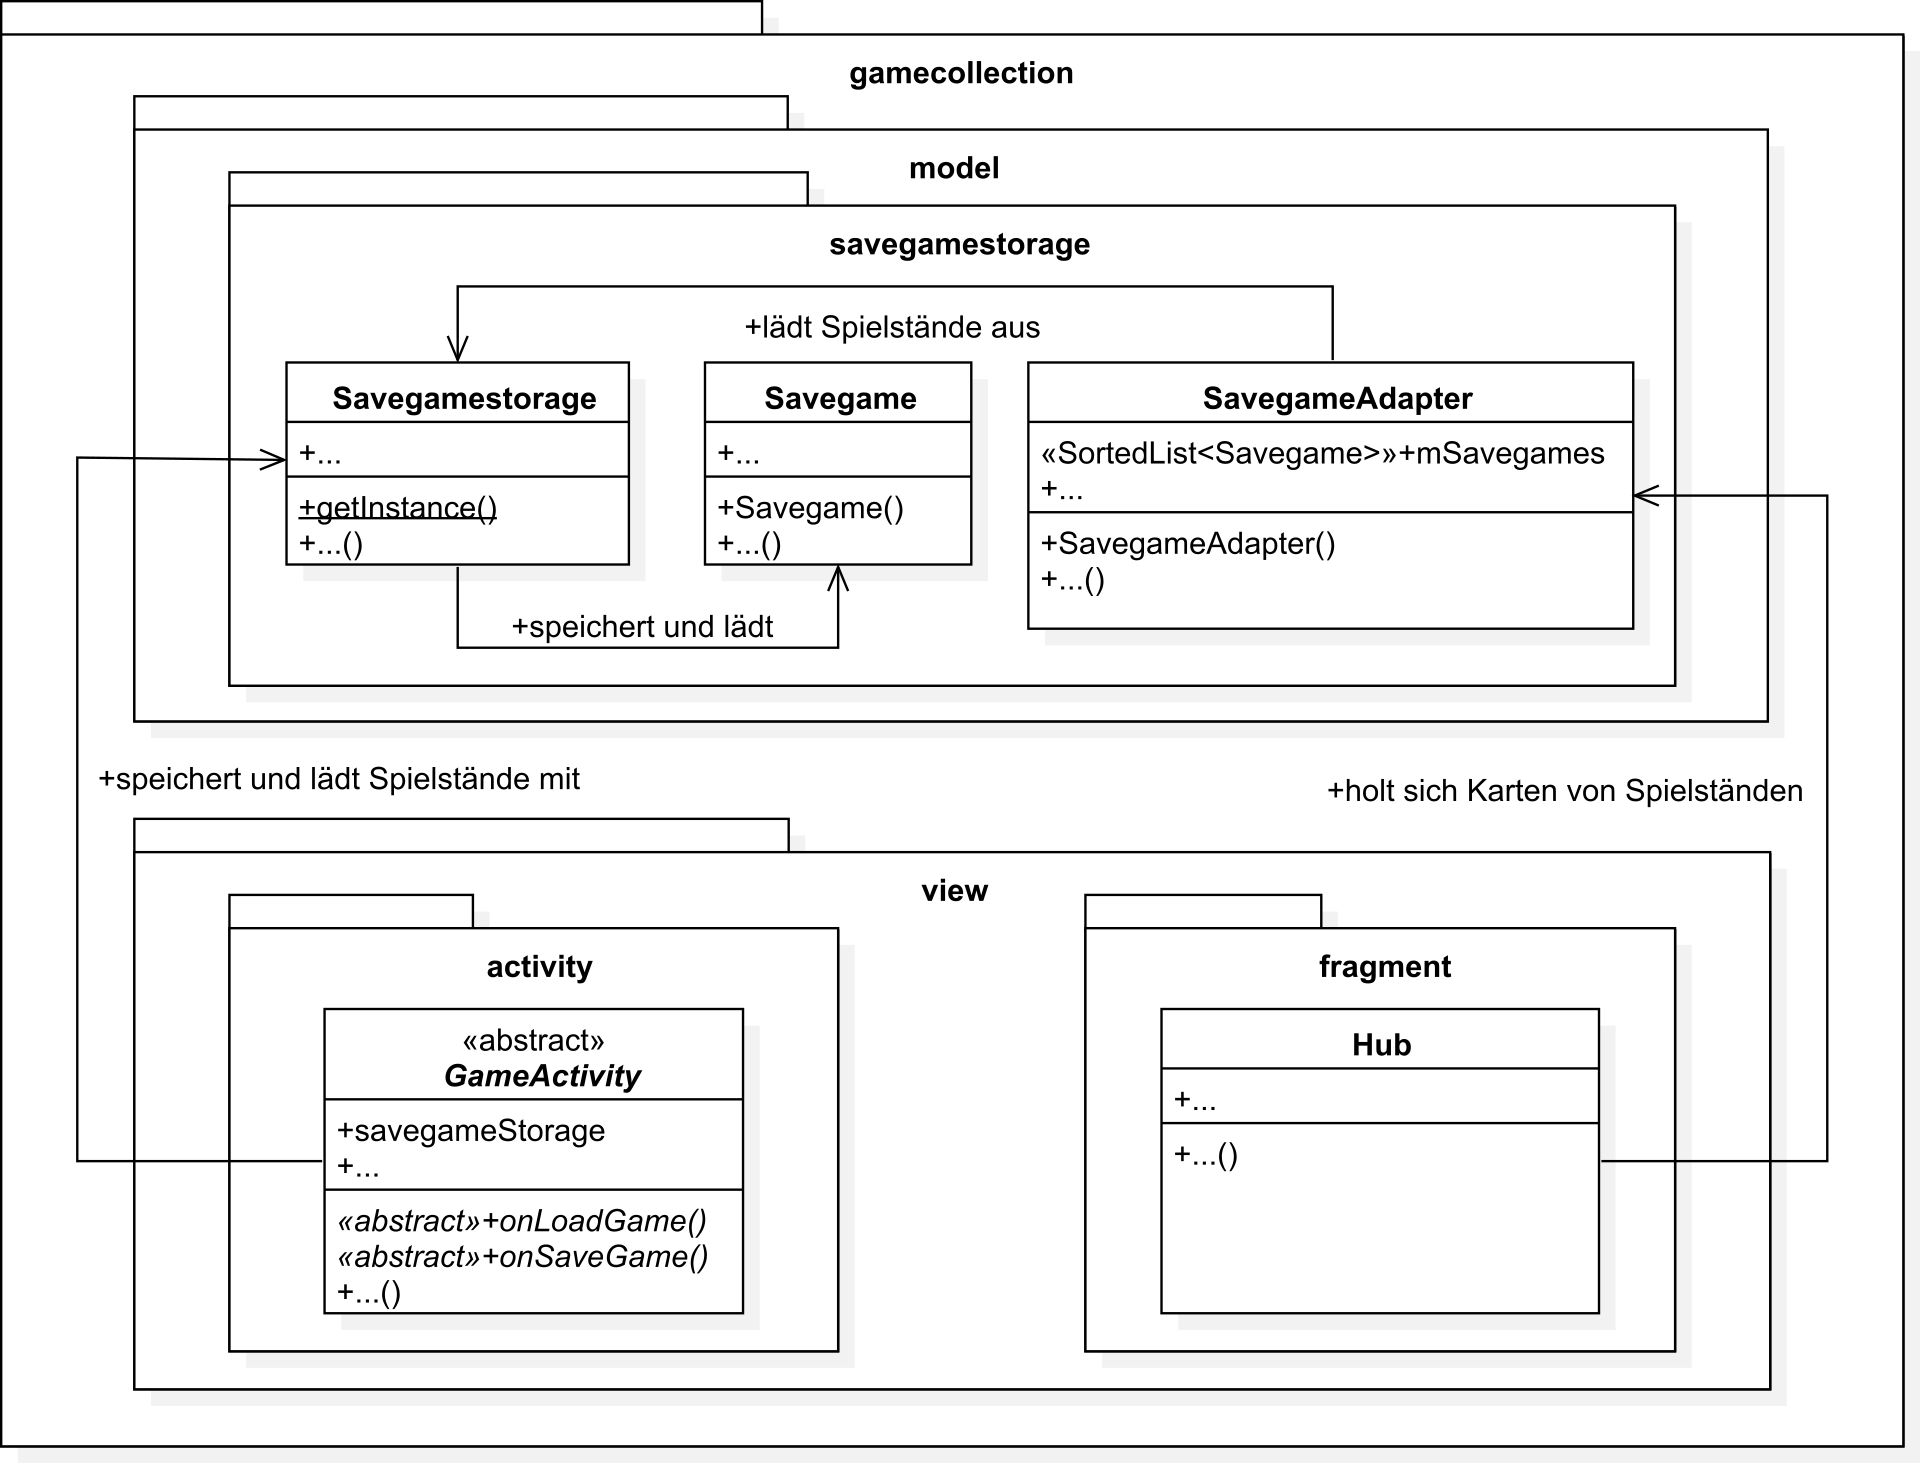
\includegraphics[width=1.0\textwidth]{resources/savegamestorage/Savegamestorage}
	\caption{Spielstand Architektur}
\end{figure}

\backmatter

%%%%%%%%%%%%%%%%%%%
%% create figure list
%%%%%%%%%%%%%%%%%%%


\listoffigures
\addcontentsline{toc}{chapter}{Verzeichnisse}			

%%%%%%%%%%%%%%%%%%%
%% create tables list
%%%%%%%%%%%%%%%%%%%
\listoftables

%%%%%%%%%%%%%%%%%%%
%% create listings list
%%%%%%%%%%%%%%%%%%%
\lstlistoflistings
\addcontentsline{toc}{chapter}{Listings}				


\printbibliography
\addcontentsline{toc}{chapter}{Literatur}				
\end{document}


